\documentclass{article}

%
\usepackage{amsmath}
\usepackage{amsthm}
\usepackage{graphicx}
\usepackage{tikz}
\usepackage{tikz-cd}
\usepackage{mathpazo}

\newtheorem{theorem}{Theorem}
\newtheorem{example}{Example}
\newtheorem{proposition}[theorem]{Proposition}
\newtheorem{lemma}[theorem]{Lemma}
\newtheorem{remark}[theorem]{Remark}


\DeclareMathOperator{\GL}{GL}
\DeclareMathOperator{\PGL}{PGL}
\DeclareMathOperator{\SL}{SL}
\DeclareMathOperator{\ad}{ad}
\newcommand{\Z}{\mathbf{Z}}
\newcommand{\Gad}{{G_{\ad}}}
\newcommand{\Gm}{\mathbf{G}_m}
\newcommand{\Gtilde}{{\tilde{G}}}
\newcommand{\Ttilde}{{\tilde{T}}}

 
\usepackage{amsmath}
\usepackage{amsthm}
\usepackage{graphicx}
\usepackage{tikz}
\usepackage{tikz-cd}
\usepackage{mathpazo}



\usepackage{tikz-3dplot}

\usepackage{geometry}
\geometry{verbose,
    tmargin=2.2cm,
    bmargin=2.2cm,
    lmargin=2.5cm,
    rmargin=2.5cm,
    headheight=3cm}


\DeclareMathOperator{\GL}{GL}
\DeclareMathOperator{\PGL}{PGL}
\DeclareMathOperator{\SL}{SL}
\DeclareMathOperator{\ad}{ad}
\newcommand{\Z}{\mathbf{Z}}
\newcommand{\Gad}{{G_{\ad}}}
\newcommand{\Gm}{\mathbf{G}_m}
\newcommand{\Gtilde}{{\tilde{G}}}
\newcommand{\Ttilde}{{\tilde{T}}}

\newtheoremstyle{note}% <name>
{10pt}% <Space above>
{3pt}% <Space below>
%{\upshape}% <Body font>
{\itshape}% <Body font>
%{\parindent}% <Indent amount>
{0pt}% <Indent amount>
{\bfseries}% <Theorem head font>
{.}% <Punctuation after theorem head>
{0.5em}% <Space after theorem headi>
{}% <Theorem head spec (can be left empty, meaning `normal')>

\theoremstyle{note}
\newtheorem{theorem}{Theorem}
\newtheorem{corollary}[theorem]{Corollary}
\newtheorem{proposition}[theorem]{Proposition}
\newtheorem{lemma}[theorem]{Lemma}
\newtheorem{rem}[theorem]{Remark}
\newtheorem{problem}[theorem]{Problem}
\newtheorem{exercise}{Exercise}[section]
\newtheorem{example}{Example}
\newtheorem{assumption}{Assumption}[section]
\newtheorem{definition}[theorem]{Definition}
\newtheorem{conjecture}[theorem]{Conjecture}


\title{\textsc{
	Michigan State University \\ 
	{\large Math 234 --  Spring 2024\\
	Lecture notes}
	}}
\date{}
\author{}

\usepackage{pgfplots}
\usepgfplotslibrary{fillbetween}
\pgfplotsset{compat=1.16,width=10cm}

\begin{document}
% \maketitle



% \input{content/08-content.tex}
% 
% Lecture 09 - 2024-01-29
\section{Cylindrical coordinates}
\begin{itemize}
    \item Cylindrical coordinates represent a point $P(x,y,z)$ in space by ordered triples $(r,\theta, z)$ in which $(r,\theta)$ is the polar coordinate of $(x,y)$.
    \item $z$ remains unchanged.
    \begin{equation*}
    \fbox{$
    \qquad
        \begin{cases}
            \begin{aligned}
                x &= r\cos \theta \\
                y &= r\sin \theta \\
                z &= z 
            \end{aligned}
        \end{cases} \qquad 
        \text{and}\qquad 
        \begin{cases}
            \begin{aligned}
                r^2 &= x^2 + y^2  \\
                \frac{y}{x} &= \tan \theta .
            \end{aligned}
        \end{cases}
        \qquad
        $}
    \end{equation*}
    \begin{center}
        \includegraphics[scale=0.7]{images/09-cylindrical.png}
    \end{center}
    \item \underline{\textbf{Example.}} Change $(x,y,z) = (-1,1,1)$ into cylindrical coordinates.
    \begin{proof} $r^2 = x^2+y^2 = 2$, thus $r=\sqrt{2}$. Then $\tan\theta = \frac{y}{x} = \frac{1}{-1} = -1$, thus $\theta = \frac{3\pi}{4}$. Hence 
    $$(-1,1,1)\mapsto \left(\sqrt{2}, \frac{3\pi}{4}, 1\right).$$
    \end{proof}
    \item \underline{\textbf{Example.}} Change $(\sqrt{2}, 3\pi/4, 2)$ to Cartesian coordinates.
    \begin{proof} We have $x = r\cos \theta = \sqrt{2}\times \left(-\frac{1}{\sqrt{2}}\right) = -1$ and $y = r\sin \theta = \sqrt{2}\times \left(\frac{1}{\sqrt{2}}\right) = 1$. Thus 
    $$(\sqrt{2}, 3\pi/4, 2)\mapsto (1,-1, 2).$$
    \end{proof}
\end{itemize}

\section{Spherical coordinates}
\begin{itemize}
    \item $(x,y,z)\mapsto (\rho, \theta,\phi)$, where basically we repeat the polar coordinate first, and the \emph{height} $z$ is tracked via the variable $\phi$, the angle with $Oz$. 
    Note that the order is sometime written as $(r,\phi, \theta)$. \textbf{Pay attention to the order!}
    \item The relations, still introducing an extra variable $r$ as in polar coordinates (it will be very useful)\color{red}
    \begin{equation*}
    \fbox{$
    \qquad
        \begin{cases}
            \begin{aligned}
                x &= (\rho \sin \phi) \cos \theta \\
                y &= (\rho \sin \phi) \sin \theta \\
                z &= \rho \cos \phi
            \end{aligned}
        \end{cases} \qquad 
        \text{and}\qquad 
        \begin{cases}
            \begin{aligned}
                 \rho^2 &= x^2+y^2+z^2 \\
                r &= \rho \sin \phi \\
                \frac{r}{z} &= \tan \phi
            \end{aligned}
        \end{cases}, \qquad \theta \in  [0,2\pi], \phi\in [0,\pi]
        \qquad
        $}
    \end{equation*}
    \begin{center}
        \includegraphics[scale=0.7]{images/09-spherical.png}
    \end{center}\color{black}
    \item If $\phi > \frac{\pi}{2}$ then $z<0$, the angle make $P$ lies below the $Oxy$-plane.
    
    \item \underline{\textbf{Example.}} Convert $(1,1,0)$ into spherical coordinate.
    \begin{proof} $\rho^2 = x^2+y^2+z^2 = 2$, thus $\rho = \sqrt{2}$. Now $z = \rho \cos \phi$ implies $0 = \sqrt{2} \cos \phi$, thus $\phi = \frac{\pi}{2}$. Finally $\tan\theta = \frac{y}{x} = 1$, thus $\theta = \frac{\pi}{4}$ (since $x>0, y>0$). We conclude 
    \begin{equation*}
        (1,1,0) \mapsto \left(\sqrt{2}, \frac{\pi}{4}, \frac{\pi}{2}\right) = (r,\theta, \phi).
    \end{equation*}
    \end{proof}

    \item \underline{\textbf{Example.}}  True/False: Consider the point with spherical coordinates $(\rho, \theta,\phi)=(4, \frac{3\pi}{4}, \frac{5\pi}{7})$. The product of the Cartesian coordinates, $xyz$, is positive.
    \begin{proof} \textbf{True}. We see that $\phi = \frac{5\pi}{7} > \frac{\pi}{2}$, thus $z<0$. Now $\theta = \frac{3\pi}{4}$, thus $x>0, y<0$ (draw a picture). Therefore $xyz>0$.
    \end{proof}
\end{itemize}
\section{Practice}
\begin{itemize}

    \item \underline{\textbf{Example.}} Convert the equation $z = \sqrt{x^2+y^2}$ into cylindrical coordinates and spherical coordinates.
    \begin{proof}\quad 
        \begin{itemize}
            \item Cylindrical: $z = r$.
            \item Spherical: $\rho \cos \phi = r = \rho \sin \phi$, thus $\tan \phi = 1$, thus $\phi = \frac{\pi}{4}$ is the equation of the cone!
        \end{itemize}
    \end{proof}
    
    \item \underline{\textbf{Example.}} Identify the surface whose equation is $z = 4-r^2$ in cylindrical coordinate.
    \begin{proof}
        We have $z = 4 - x^2-y^2$, thus this is a elliptical paraboloid (one term of 1st order, two terms of second order having the same sign).
    \end{proof}

    \item \underline{\textbf{Example.}} Convert to $x,y,z$ the surface: $\rho = \sin \phi\cos \phi$.
    \begin{proof} We can do 
    \begin{equation*}
        (x^2+y^2+z^2)^\frac{3}{2}= \rho^3 = (\rho \sin \phi) (\rho\cos \phi) = rz = z\sqrt{x^2+y^2}.
    \end{equation*}
    The answer is $(x^2+y^2+z^2)^\frac{3}{2} = z\sqrt{x^2+y^2}$.
    \end{proof}

    \item \underline{\textbf{Example.}} Identify the surface whose equation is: $\rho = \sin \phi\cos \theta$.
    \begin{proof} We can do 
    \begin{equation*}
        x^2+y^2+z^2 =\rho^2 = (\rho \sin \phi) \cos \theta = r\cos\theta = x
    \end{equation*}
    Therefore 
    \begin{equation*}
        \left(x-\frac{1}{2}\right)^2 + y^2 +z^2 = \frac{1}{4}
    \end{equation*}
    This is a sphere centered at $(\frac{1}{2},0,0)$ with radius $\frac{1}{2}$, this is a \emph{ellipsoid}.
    \end{proof}
\end{itemize}
% 
% Lecture 10 - 2024-01-31
\section{Cylindrical coordinates}
\begin{itemize}
    \item Cylindrical coordinates represent a point $P(x,y,z)$ in space by ordered triples $(r,\theta, z)$ in which $(r,\theta)$ is the polar coordinate of $(x,y)$.
    \item $z$ remains unchanged.
    \begin{equation*}
    \fbox{$
    \qquad
        \begin{cases}
            \begin{aligned}
                x &= r\cos \theta \\
                y &= r\sin \theta \\
                z &= z 
            \end{aligned}
        \end{cases} \qquad 
        \text{and}\qquad 
        \begin{cases}
            \begin{aligned}
                r^2 &= x^2 + y^2  \\
                \frac{y}{x} &= \tan \theta .
            \end{aligned}
        \end{cases}
        \qquad
        $}
    \end{equation*}
    \begin{center}
        \includegraphics[scale=0.7]{content/09-cylindrical.png}
    \end{center}
    \item \underline{\textbf{Example.}} Change $(x,y,z) = (-1,1,1)$ into cylindrical coordinates.
    \begin{proof} $r^2 = x^2+y^2 = 2$, thus $r=\sqrt{2}$. Then $\tan\theta = \frac{y}{x} = \frac{1}{-1} = -1$, thus $\theta = \frac{3\pi}{4}$. Hence 
    $$(-1,1,1)\mapsto \left(\sqrt{2}, \frac{3\pi}{4}, 1\right).$$
    \end{proof}
    \item \underline{\textbf{Example.}} Change $(\sqrt{2}, 3\pi/4, 2)$ to Cartesian coordinates.
    \begin{proof} We have $x = r\cos \theta = \sqrt{2}\times \left(-\frac{1}{\sqrt{2}}\right) = -1$ and $y = r\sin \theta = \sqrt{2}\times \left(\frac{1}{\sqrt{2}}\right) = 1$. Thus 
    $$(\sqrt{2}, 3\pi/4, 2)\mapsto (1,-1, 2).$$
    \end{proof}
\end{itemize}

\section{Spherical coordinates}
\begin{itemize}
    \item $(x,y,z)\mapsto (\rho, \theta,\phi)$, where basically we repeat the polar coordinate first, and the \emph{height} $z$ is tracked via the variable $\phi$, the angle with $Oz$. 
    Note that the order is sometime written as $(r,\phi, \theta)$. \textbf{Pay attention to the order!}
    \item The relations, still introducing an extra variable $r$ as in polar coordinates (it will be very useful)\color{red}
    \begin{equation*}
    \fbox{$
    \qquad
        \begin{cases}
            \begin{aligned}
                x &= (\rho \sin \phi) \cos \theta \\
                y &= (\rho \sin \phi) \sin \theta \\
                z &= \rho \cos \phi
            \end{aligned}
        \end{cases} \qquad 
        \text{and}\qquad 
        \begin{cases}
            \begin{aligned}
                 \rho^2 &= x^2+y^2+z^2 \\
                r &= \rho \sin \phi \\
                \frac{r}{z} &= \tan \phi
            \end{aligned}
        \end{cases}, \qquad \theta \in  [0,2\pi], \phi\in [0,\pi]
        \qquad
        $}
    \end{equation*}
    \begin{center}
        \includegraphics[scale=0.7]{content/09-spherical.png}
    \end{center}\color{black}
    \item If $\phi > \frac{\pi}{2}$ then $z<0$, the angle make $P$ lies below the $Oxy$-plane.
    
    \item \underline{\textbf{Example.}} Convert $(1,1,0)$ into spherical coordinate.
    \begin{proof} $\rho^2 = x^2+y^2+z^2 = 2$, thus $\rho = \sqrt{2}$. Now $z = \rho \cos \phi$ implies $0 = \sqrt{2} \cos \phi$, thus $\phi = \frac{\pi}{2}$. Finally $\tan\theta = \frac{y}{x} = 1$, thus $\theta = \frac{\pi}{4}$ (since $x>0, y>0$). We conclude 
    \begin{equation*}
        (1,1,0) \mapsto \left(\sqrt{2}, \frac{\pi}{4}, \frac{\pi}{2}\right) = (r,\theta, \phi).
    \end{equation*}
    \end{proof}

    \item \underline{\textbf{Example.}}  True/False: Consider the point with spherical coordinates $(\rho, \theta,\phi)=(4, \frac{3\pi}{4}, \frac{5\pi}{7})$. The product of the Cartesian coordinates, $xyz$, is positive.
    \begin{proof} \textbf{True}. We see that $\phi = \frac{5\pi}{7} > \frac{\pi}{2}$, thus $z<0$. Now $\theta = \frac{3\pi}{4}$, thus $x>0, y<0$ (draw a picture). Therefore $xyz>0$.
    \end{proof}
\end{itemize}
\section{Practice}
\begin{itemize}

    \item \underline{\textbf{Example.}} Convert the equation $z = \sqrt{x^2+y^2}$ into cylindrical coordinates and spherical coordinates.
    \begin{proof}\quad 
        \begin{itemize}
            \item Cylindrical: $z = r$.
            \item Spherical: $\rho \cos \phi = r = \rho \sin \phi$, thus $\tan \phi = 1$, thus $\phi = \frac{\pi}{4}$ is the equation of the cone!
        \end{itemize}
    \end{proof}
    
    \item \underline{\textbf{Example.}} Identify the surface whose equation is $z = 4-r^2$ in cylindrical coordinate.
    \begin{proof}
        We have $z = 4 - x^2-y^2$, thus this is a elliptical paraboloid (one term of 1st order, two terms of second order having the same sign).
    \end{proof}

    \item \underline{\textbf{Example.}} Convert to $x,y,z$ the surface: $\rho = \sin \phi\cos \phi$.
    \begin{proof} We can do 
    \begin{equation*}
        (x^2+y^2+z^2)^\frac{3}{2}= \rho^3 = (\rho \sin \phi) (\rho\cos \phi) = rz = z\sqrt{x^2+y^2}.
    \end{equation*}
    The answer is $(x^2+y^2+z^2)^\frac{3}{2} = z\sqrt{x^2+y^2}$.
    \end{proof}

    \item \underline{\textbf{Example.}} Identify the surface whose equation is: $\rho = \sin \phi\cos \theta$.
    \begin{proof} We can do 
    \begin{equation*}
        x^2+y^2+z^2 =\rho^2 = (\rho \sin \phi) \cos \theta = r\cos\theta = x
    \end{equation*}
    Therefore 
    \begin{equation*}
        \left(x-\frac{1}{2}\right)^2 + y^2 +z^2 = \frac{1}{4}
    \end{equation*}
    This is a sphere centered at $(\frac{1}{2},0,0$ with radius $\frac{1}{2}$, this is a \emph{ellipsoid}.
    \end{proof}
\end{itemize}
% % Lecture 11 - 2024-02-02
\section{Function of several variables}
\begin{definition}\quad 
\begin{itemize}
    \item[(a)] A function of two variables is a rule that assigns to each ordered pair of real numbers $(x,y)$ in a set $D$ a unique real number denoted by $f(x,y)$. The set $D$ is the domain of $f$ and its range is the set of values that $f$ takes on, that is, $\{f(x,y):(x,y)\in D\}$.
    \item[(b)] We often write $z=f(x,y)$.
    \item[(c)] The graph of $z=f(x,y)$ is the set of all points $(x,y,z)\in \mathbb{R}^3$ such that $z = f(x,y)$ and $(x,y)\in D$.
\end{itemize}
\end{definition}

\begin{example} Consider $f(x,y) = \sqrt{16-x^2-y^2}$. Sketch the domain of $f$. Graph $z=f(x,y)$ using traces of $z=0, x=0, y=0$.
\end{example}
\begin{proof} The domain us $D = \{(x,y)\in \mathbb{R}^2: 16-x^2-y^2\geq 0\} =  \{(x,y)\in \mathbb{R}^2: x^2+y^2 \leq 4^2\}$. This is the (closed) circle centered at $(0,0)$ with radius $4$. The trace of $z=0, y=0, x=0$ give us $x^2+y^2 = 16$, $z^2+y^2=16$ and $z^2+x^2=16$, i.e., in any cross-section it is a circle, therefore the graph of this function is a sphere of radius $4$ in $\mathbb{R}^3$ (but only half of the sphere, the upper half as $z\geq 0$). 
\begin{center}
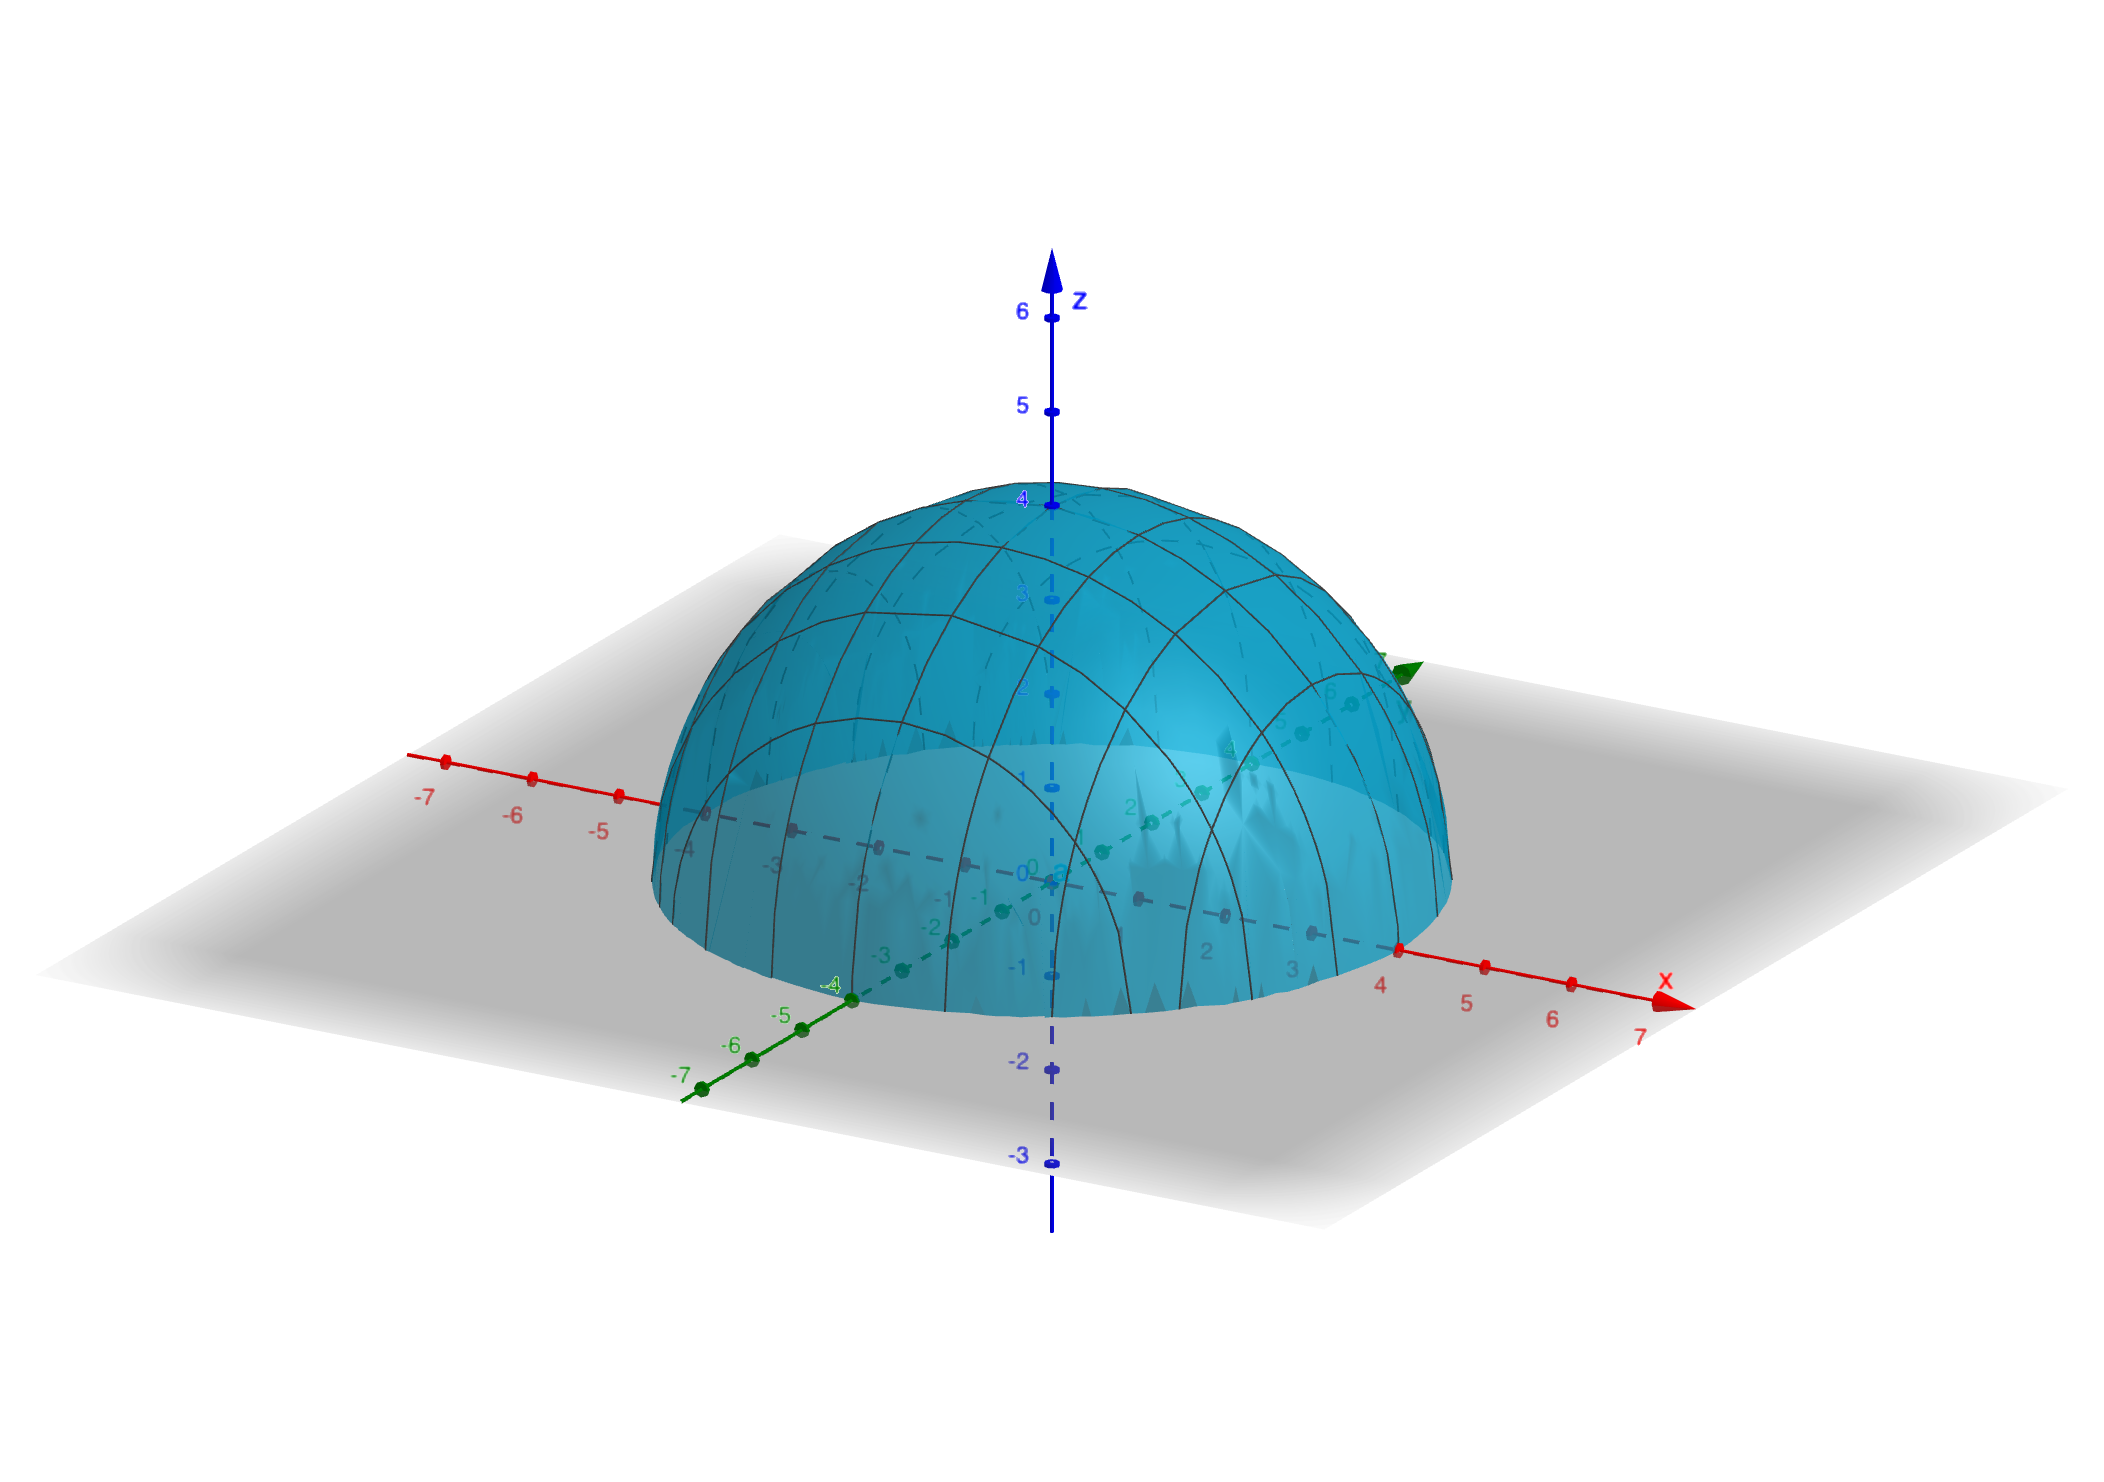
\includegraphics[scale=0.1]{images/11-ex1.png}    
\end{center}    
\end{proof}

\begin{definition} The contours of a function $f$ of two variables are the curves with equations $f(x,y) = k$, where $k$ is constant (in the range of $f$).
\end{definition}

\begin{example} Sketch the level curves of $f(x,y) = \frac{1}{x^2+y^2}$, with $k=\frac{1}{9}, \frac{1}{4}, 1, 4, 9$. Use these to attempt to sketch a 3D version of the graph.
\end{example}
\begin{proof} With $k=\frac{1}{3}$ we have $f(x,y) = \frac{1}{9}$ is equivalent to $x^2+y^2 = 3^2$, it is a cirlce. Similarly with $k=\frac{1}{4}$ it is a circle $x^2+y^2=4$. We have a set of cirles centered at $(0,0)$ with radius $3,2,1,\frac{1}{2}, \frac{1}{3}$, correspondingly to $k=\frac{1}{9}, \frac{1}{4}, 1, 4, 9$.
\clearpage
\begin{center}
    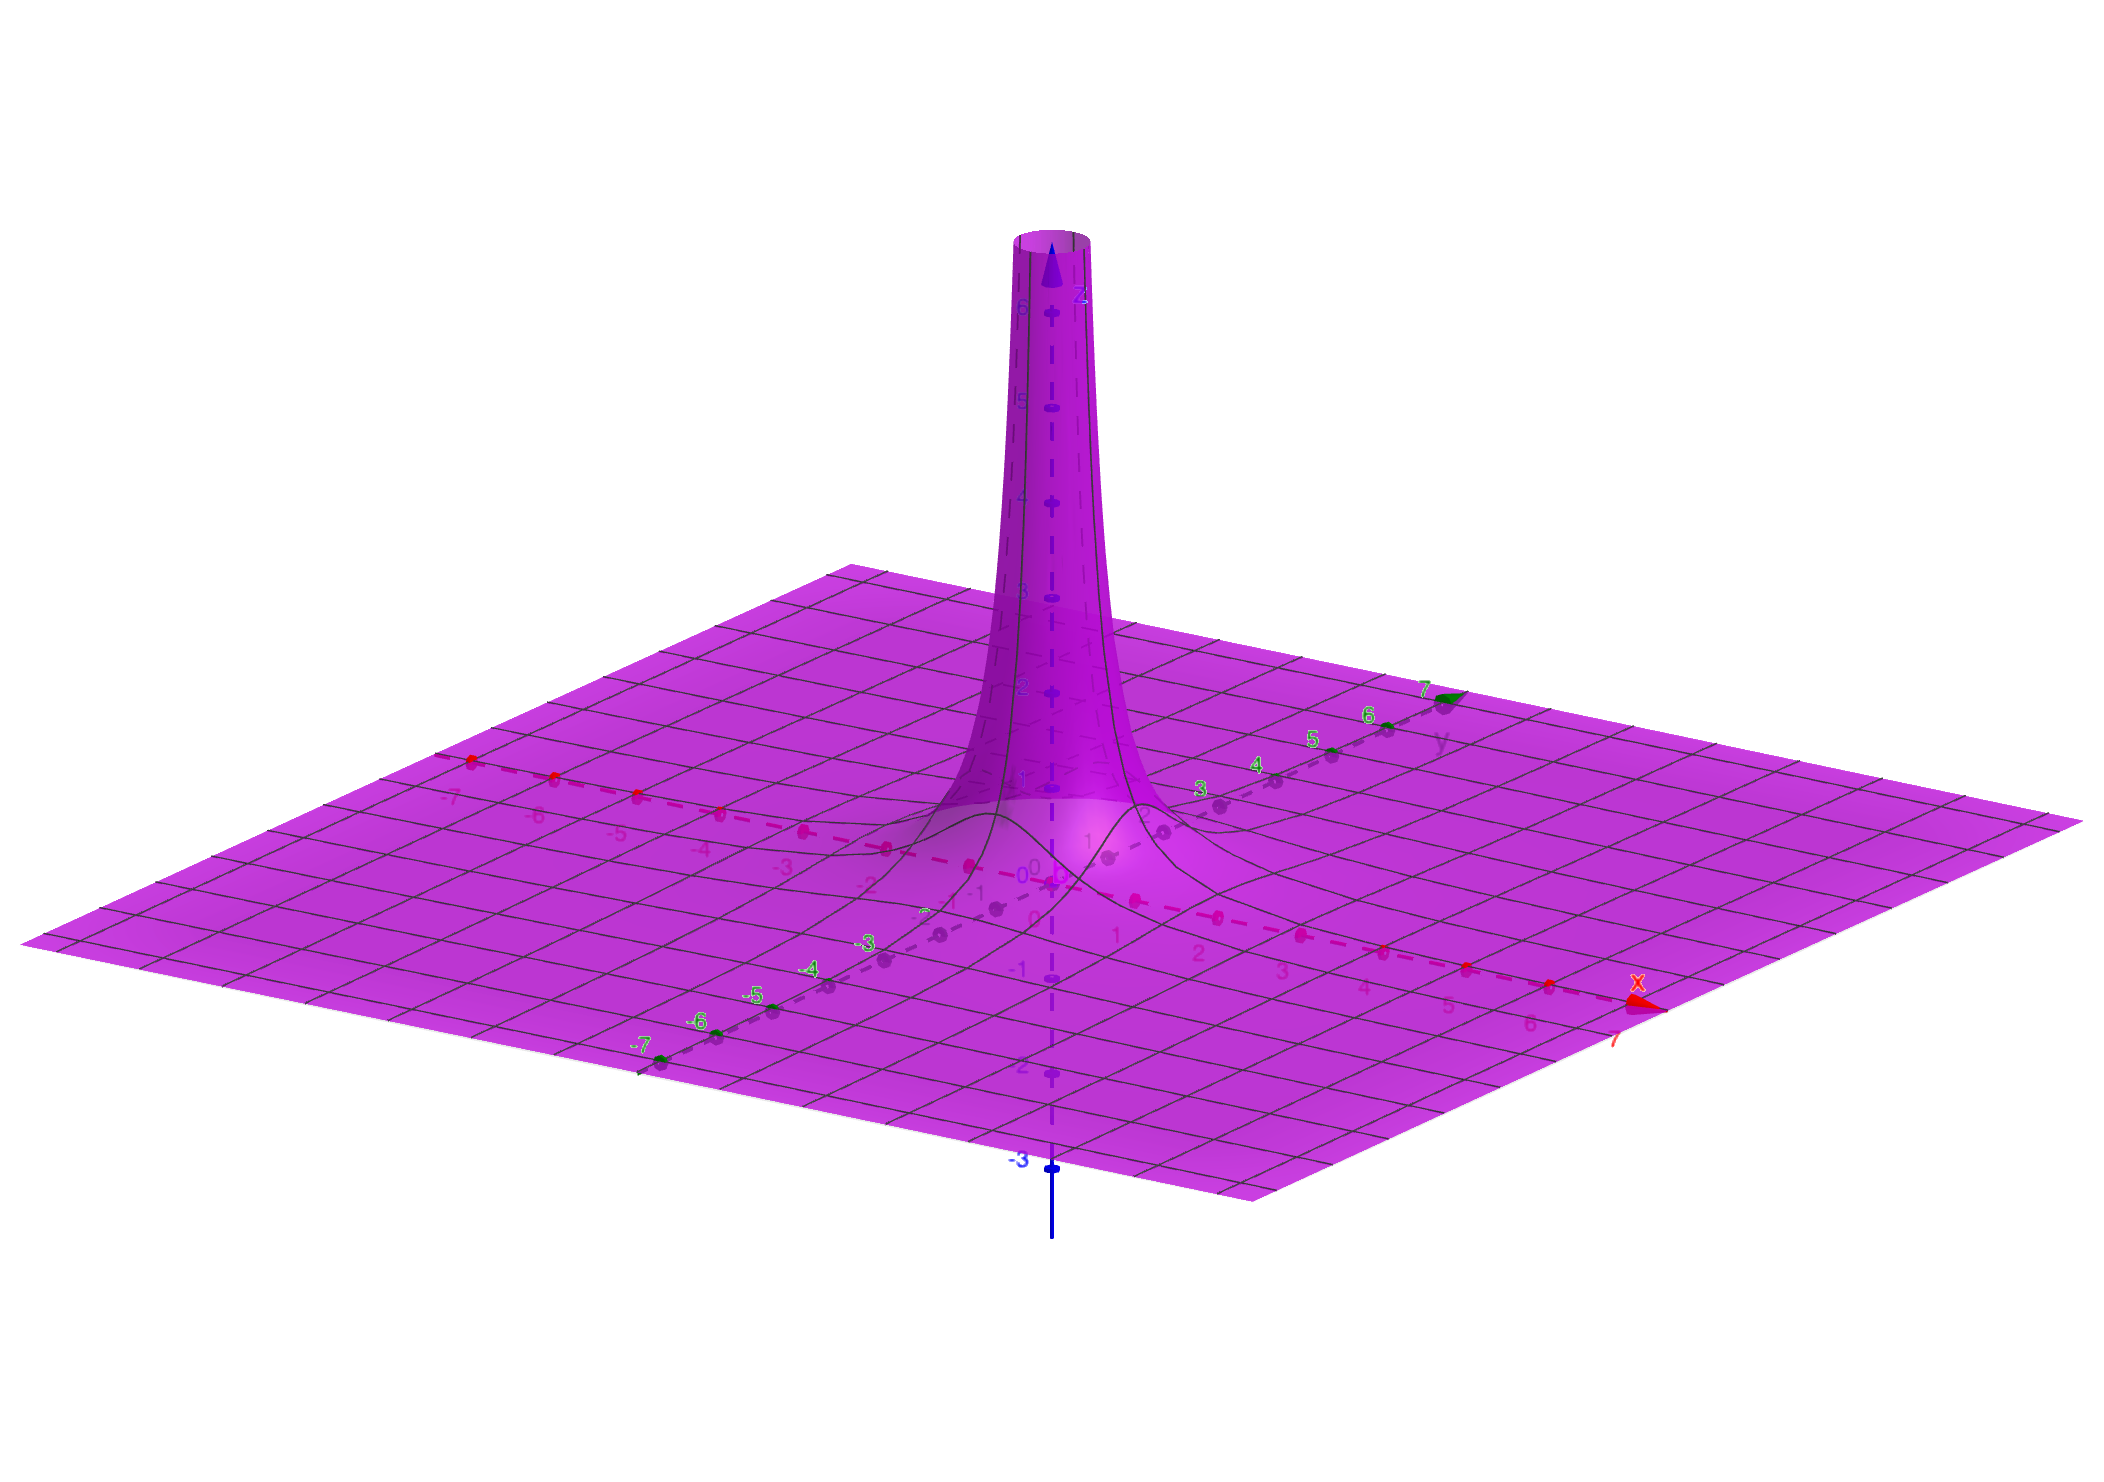
\includegraphics[scale=0.1]{images/11-ex2-a.png} \quad 
    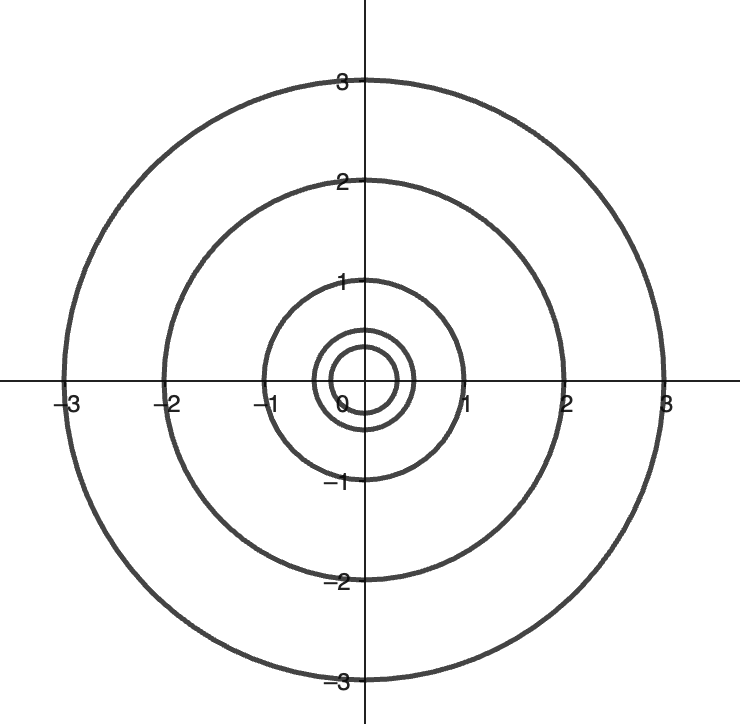
\includegraphics[scale=0.5]{images/11-ex2-b.png}    
\end{center}
Note: if $f(x,y)$ is a 2-variables function then $\mathrm{graph}(f)$ is 3D (on the left), but its contours are 2D as in the picture (on the right).
\end{proof}


\begin{definition} A function of 3 variables is $f(x,y,z)$ from a domain $D\subset \mathbb{R}^3$ to $\mathbb{R}$. The \textbf{level surfaces} of $f(x,y,z)$ are the surfaces with the equation $f(x,y,z) = k$ where $k$ is a constant (by looking at level surfaces, we can view it in 3D, instead of the graph of $f$ is in 4D).
\end{definition}

\begin{example} Find the domain of $f(x,y) = \frac{(x-1)(y+2)}{(y-x)(y-x^3)}$. Sketch and write the domain in set notation.
\end{example}
\begin{proof} $D=\{(x,y)\in \mathbb{R}^2: y\neq x, y\neq x^3\}$. The domain is the whole plane $\mathbb{R^2}$ (the $xy$-plane) removing the line $y=x$ and the curve $y=x^3$.

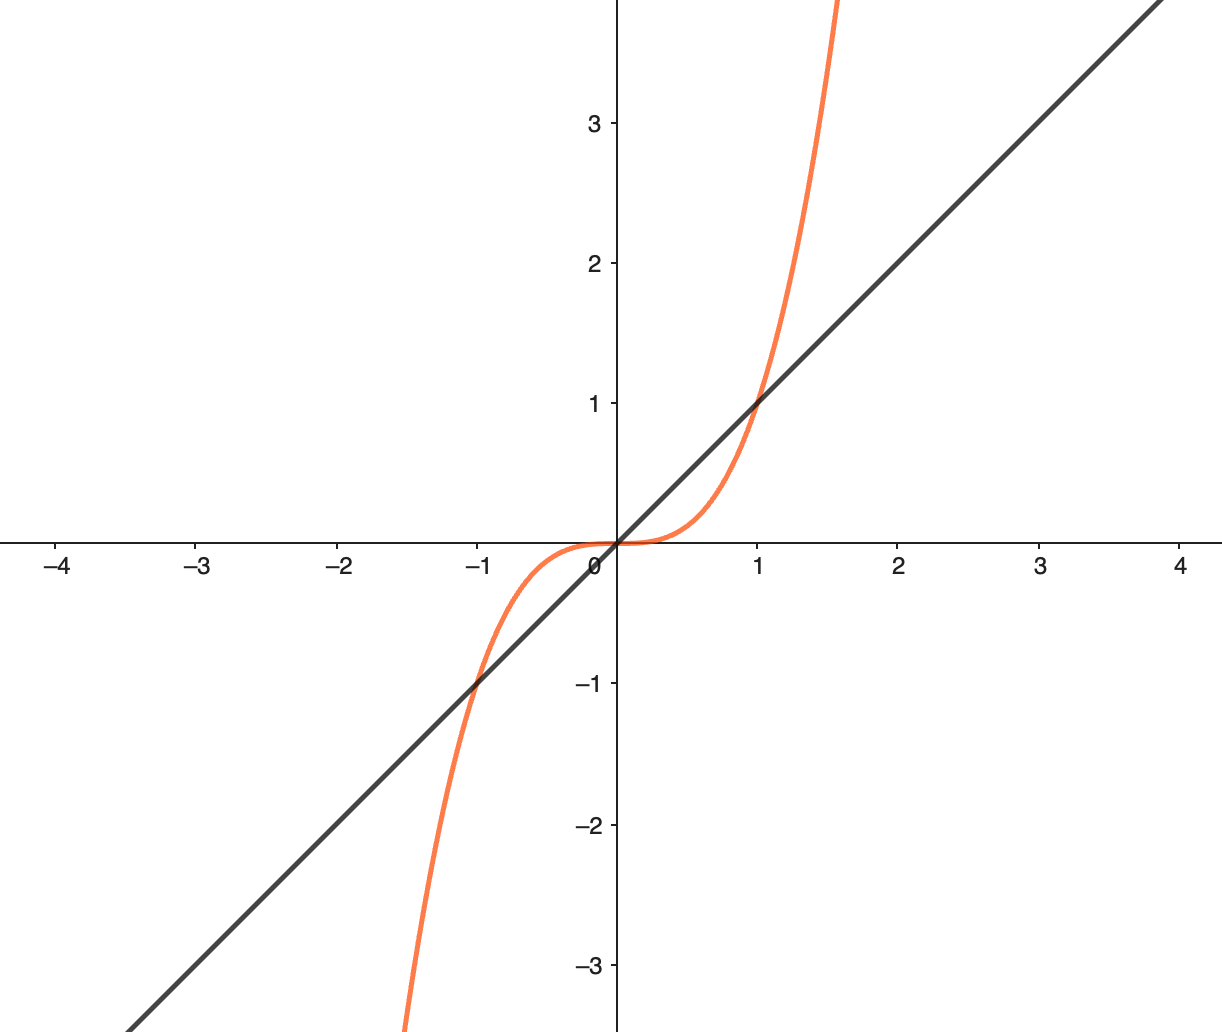
\includegraphics[scale=0.6]{images/11-ex3.png}    

\end{proof}

\begin{example} Consider the function $z=f(x,y) = \sqrt{y-x}$.
    \begin{itemize}
        \item[(a)] Dmain $D = \{(x,y): y-x\geq 0\}=\{(x,y): y\geq x\}$. (The line $y=x$ is included.)
        \begin{center}
            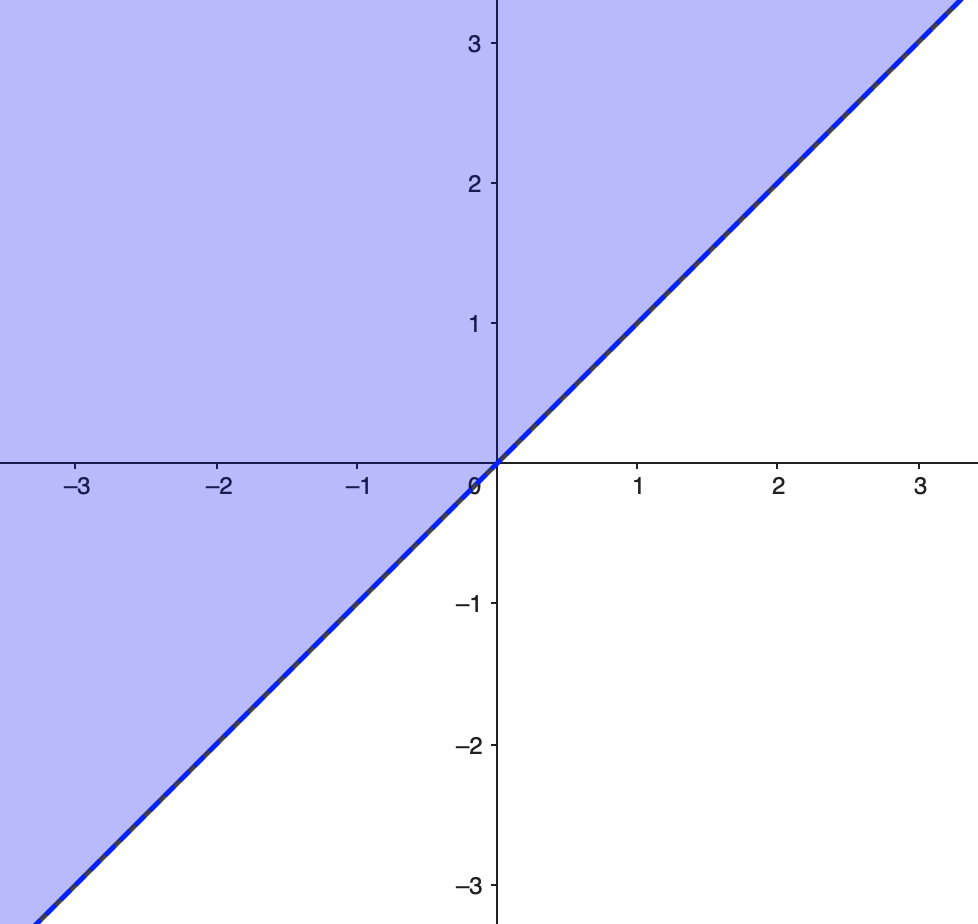
\includegraphics[scale=0.3]{images/11-ex4-a.png}
        \end{center}
        \item[(b)] The range is $z\in [0,+\infty)$.
        \item[(c)] Sketch some level curves and the graph
        \begin{center}
            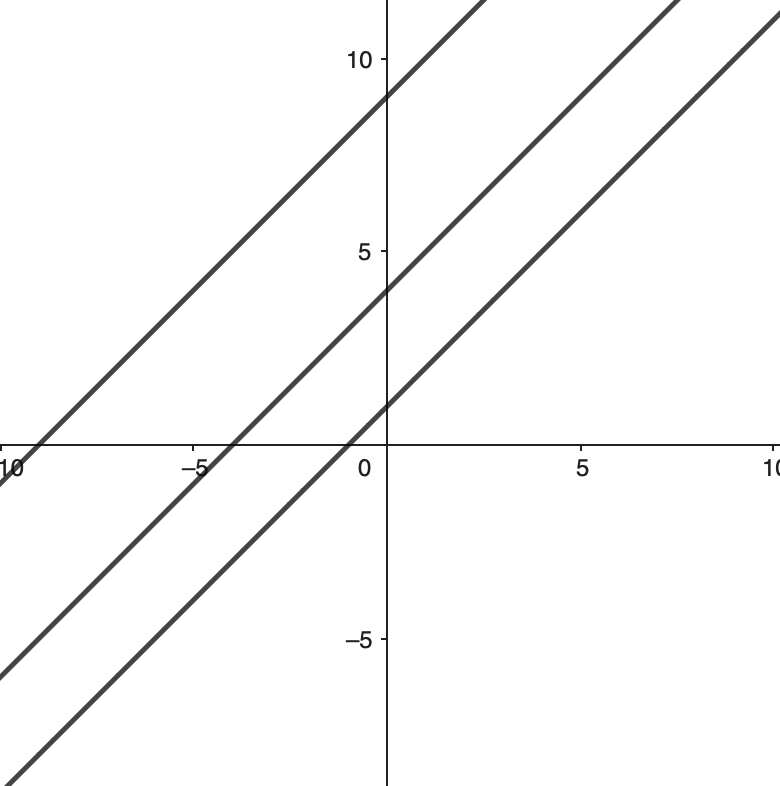
\includegraphics[scale=0.4]{images/11-ex4-b.png}\quad 
            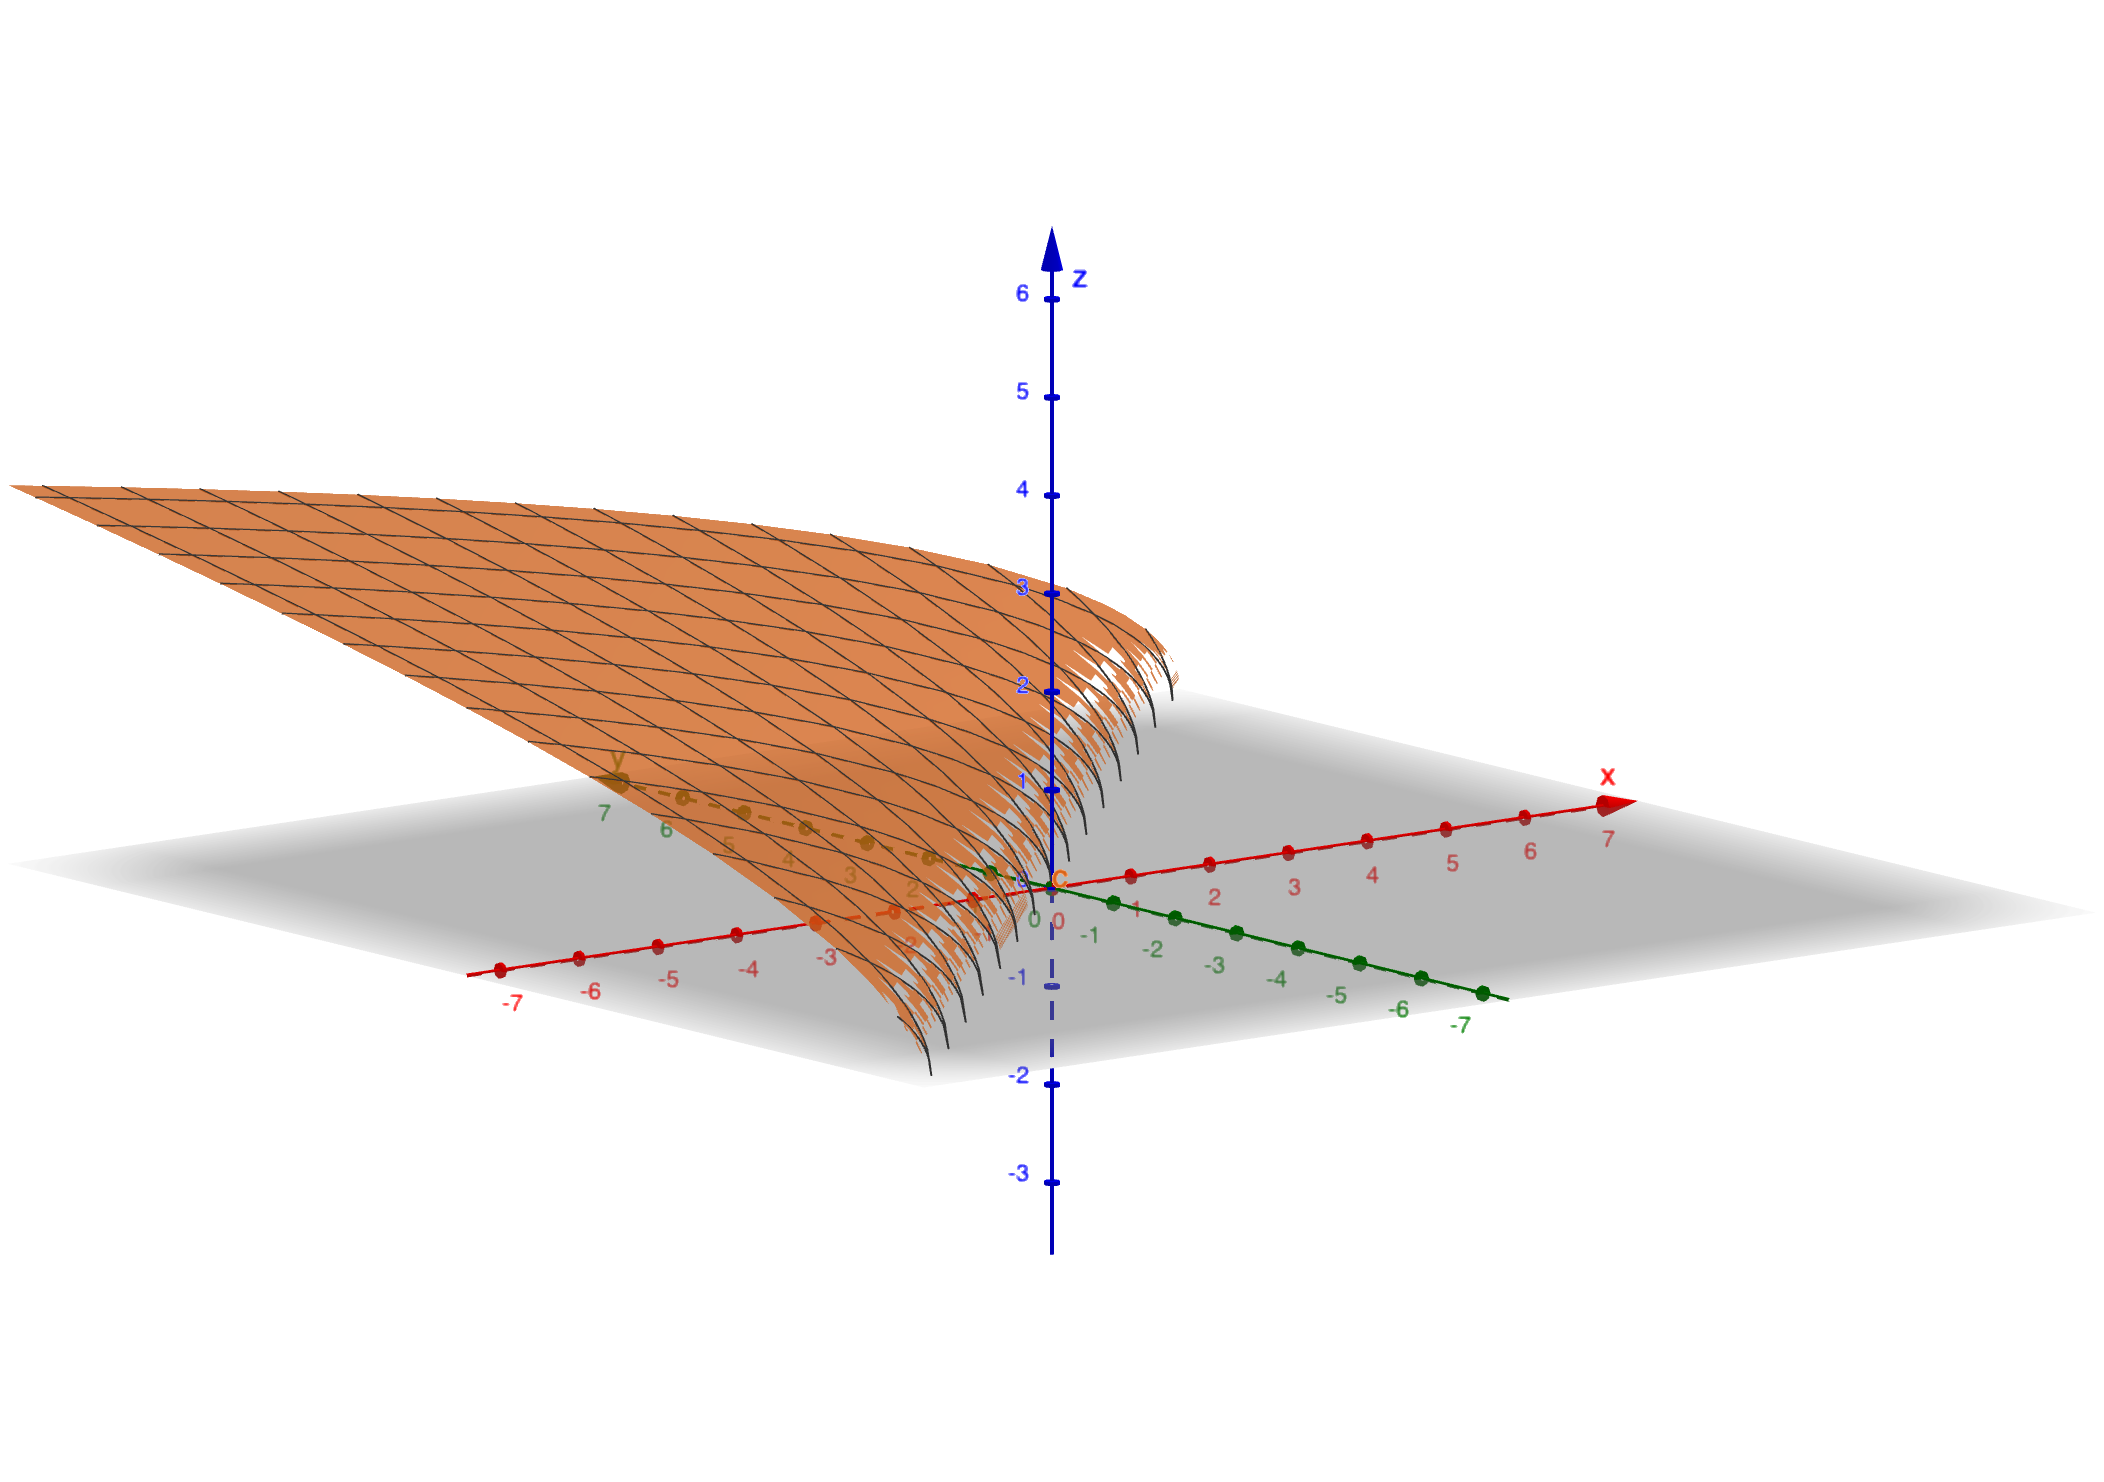
\includegraphics[scale=0.1]{images/11-ex4-c.png}
        \end{center}
    \end{itemize}
\end{example}


\section{Partial derivatives}

\begin{definition}[Partial Derivatives]\quad 
    \begin{itemize}
        \item[(a)] The partial derivatives of $f(x,y)$ with respect to $x$ at $(a,b)$ is denoted by $f_x(a,b)$ and is given by
        \begin{equation*}
            f_x(a,b) = \lim_{h\to 0} \frac{f(a+h,b) - f(a,b)}{|h|}. 
        \end{equation*}
        This is equivalent to considering $y$ as a constant and taking derivative in $x$.
        \item[(b)] The partial derivatives of $f(x,y)$ with respect to $y$ at $(a,b)$ is denoted by $f_y(a,b)$ and is given by
        \begin{equation*}
            f_y(a,b) = \lim_{k\to 0} \frac{f(a,b+k) - f(a,b)}{|k|}. 
        \end{equation*}
        This is equivalent to considering $x$ as a constant and taking derivative in $y$.
        \item[(c)] Other notations
        \begin{align*}
            f_x(x,y) &= f_x = \frac{\partial f}{\partial x} = \frac{\partial f}{\partial x}(x,y) = \frac{\partial z}{\partial x} = D_xf \\
            f_y(x,y) &= f_y = \frac{\partial f}{\partial y} = \frac{\partial f}{\partial y}(x,y) = \frac{\partial z}{\partial y} = D_yf .
        \end{align*}
        \item[(d)] Second-order derivatives:
        \begin{align*}
            (f_x)_x &= f_{xx} = \frac{\partial }{\partial x}\left(\frac{\partial f}{\partial x}\right) = \frac{\partial^2 f}{\partial x^2} = \frac{\partial^2 z}{\partial x^2} \\
            (f_y)_y &= f_{yy} = \frac{\partial }{\partial y}\left(\frac{\partial f}{\partial y}\right) = \frac{\partial^2 f}{\partial y^2} = \frac{\partial^2 z}{\partial y^2} \\
            (f_x)_y &= f_{xy} = \frac{\partial }{\partial y}\left(\frac{\partial f}{\partial x}\right) = \frac{\partial^2 f}{\partial y \partial x} = \frac{\partial^2 z}{\partial y \partial x} \\
            (f_y)_x &= f_{yx} = \frac{\partial }{\partial x}\left(\frac{\partial f}{\partial y}\right) = \frac{\partial^2 f}{\partial x \partial y} = \frac{\partial^2 z}{\partial x \partial y} .
        \end{align*}
        Note the sequence: the first derivative is taken closest to the function.
        \item[(e)] (Clairaut's Theorem) The order of taking derivatives (around a point $(a,b)$) does not matter if the second order derivaties are continuous and defined around a point $(a,b)$. 
        \begin{equation*}
            \frac{\partial }{\partial x} \frac{\partial f}{\partial y}(a,b) = \frac{\partial }{\partial y} \frac{\partial f}{\partial x}(a,b).
        \end{equation*}
        \item[(f)] The gradient
        \begin{equation*}
            \nabla f(a,b) = \left(f_x(a,b), f_y(a,b)\right)
        \end{equation*}
        gives the direction in which the value of the function increases the fastest.
    \end{itemize}
\end{definition}
\begin{example} We have
    \begin{align*}
        &\frac{\partial}{\partial x} \left(\frac{\partial}{\partial y} \left(xy + x\sin y + \frac{y}{x}\right)\right) =  \frac{\partial}{\partial x} \left(x + x\cos y + \frac{1}{x}\right) = 1 + \cos y -\frac{1}{x^2}\\
        &\frac{\partial}{\partial y} \left(\frac{\partial}{\partial x} \left(xy + x\sin y + \frac{y}{x}\right)\right) =  \frac{\partial}{\partial y} \left(y + \sin y - \frac{y}{x^2}\right) = 1 + \cos y -\frac{1}{x^2}\\
    \end{align*}
\end{example}

\begin{example} Let $v(x,y) = \frac{xy}{x-y}$. Compute $v_x, v_{xx}, v_{xy}$.
\end{example}
\begin{proof} We use product rule or quotient rule, or any rule from Calculus 1 and 2:
\begin{align*}
    v_x = \frac{y(x-y) - xy}{(x-y)^2} = \frac{-y^2}{(x-y)^2}, \qquad v_{xx} = \frac{- (-y^2)2(x-y)}{(x-y)^4} = \frac{2y^2}{(x-y)^3}\\
    v_{xy} = \frac{-2y(x-y)^2 - (-y^2)2(x-y)}{(x-y)^4} = \frac{-2y+2y^2}{(x-y)^3}.
\end{align*}
\end{proof}

\begin{example} Find $f_{xyz}$ for $f(x,y,z)= xyz + (x^2+y^2) \frac{\sin^{-1}(x\sqrt{y})}{\tan(x)}$. 
\end{example}
\begin{proof} Note that $\frac{\partial}{\partial x}(\sin^{-1}(x)) = \frac{\partial}{\partial x}(\arcsin(x)) = \frac{1}{\sqrt{1-x^2}}$. We compute (product rule, then quotient rule)
\begin{align*}
    f_x = yz + 2x \frac{\partial }{\partial x} \left((x^2+y^2) \frac{\sin^{-1}(x\sqrt{y})}{\tan(x)}\right).
\end{align*}
Let us not computing the derivative of that term for now, for a reason we will see soon. Now we have
\begin{align*}
    f_{xy} = \frac{\partial}{\partial y} f_x 
    &= \frac{\partial}{\partial y} (yz) + \frac{\partial}{\partial y}\left[2x \frac{\partial }{\partial x} \left((x^2+y^2) \frac{\sin^{-1}(x\sqrt{y})}{\tan(x)}\right)\right] \\
    &= z + \frac{\partial}{\partial y}\left[2x \frac{\partial }{\partial x} \left((x^2+y^2) \frac{\sin^{-1}(x\sqrt{y})}{\tan(x)}\right)\right].
\end{align*}
Now we have
\begin{align*}
    f_{xyz} = 1 + \frac{\partial}{\partial z} \underbrace{\frac{\partial}{\partial y}\left[2x \frac{\partial }{\partial x} \left((x^2+y^2) \frac{\sin^{-1}(x\sqrt{y})}{\tan(x)}\right)\right]}_{\text{no $z$ involved, thus this term is}\;0 }.
\end{align*}
The intergral is zero, since there is no $z$ involved, and we treat $x,y$ as constants when taking $\frac{\partial}{\partial z}$.
\end{proof}

\begin{example} Suppose you are surrounded by bees given by the bee density function
\begin{equation*}
    B(x,y) = 100-x^2+y^2+3y \qquad \text{bees}/\text{unit}^2.
\end{equation*}
You are currently standing at $(1,1)$. Which of the four directions would be best to run in $\{\textbf{i},-\textbf{i}, \textbf{j}, -\textbf{j}\}$?
\end{example}
\begin{proof} We have
    \begin{align*}
        \nabla B(x,y) = (-2x, 2y+3) \qquad \Longrightarrow\qquad \nabla B(1,1) = (-2, 5).
    \end{align*}
    The best direction to run would be the opposite of $(-2,5)$, i.e, $\textbf{v} = (2,-5)$. Now among the 4 directions, we choose the one that is closest, i.e., taking the dot product to find the one with smallest angle, i.e., $\cos \theta$ the biggest:
    \begin{itemize}
        \item For $\textbf{i} = (1,0)$ then $(1,0)\cdot(2,-5) = 2$.
        \item For $-\textbf{i} = (-1,0)$ then $(-1,0)\cdot(2,-5) = -2$.
        \item For $\textbf{j} = (0,1)$ then $(0,1)\cdot(2,-5) = -5$.
        \item For $-\textbf{j} = (0,-1)$ then $(0,-1)\cdot(2,-5) = 5$.
    \end{itemize}
    Therefore we choose $-\textbf{j}$.
\end{proof}
% \section{Tangent planes}
% \begin{definition}
% \begin{itemize}
%     \item The tangent plane to the surface $z=f(x,y)$ at the point $P(x_0,y_0,z_0)$ is defined to be the plane 
% \end{itemize}    
% \end{definition}
% \clearpage

\begin{example} Find equation of the tangent plane of the surface $z=f(x,y) = 3y^2-2x^2+x$ at the point $(2,-1,3)$.
\end{example}
\begin{proof} \quad 
\begin{itemize}
    \item Step 1. We write the general form
    \begin{equation*}
        z - z_0 = f_x(x_0,y_0)(x-x_0) + f_y(x_0,y_0)(y-y_0).
    \end{equation*}
    \item Step 2. Plug in $(x_0,y_0,z_0) = (2,-1,-3)$
    \begin{align*}
         z - (-3) &= f_x(2,-1)(x-2) + f_y(2,-1)(y-(-1)).  \\
         z + 3 &= f_x(2,-1)(x-2) + f_y(2,-1)(y+1). 
    \end{align*}
    \item Step 3. Compute the partial derivatives
    \begin{align*}
        f_x(x,y) = -4x+1, \qquad f_x(2,-1) = -7\\
        f_y(x,y) = 6y, \qquad f_y(2,-1) = -6.
    \end{align*}
    \item Step 4. Final answer
    \begin{equation*}
        z + 3 = -7(x-2) - 6 (y+1).
    \end{equation*}
\end{itemize}
\end{proof}
\clearpage 

\begin{example} Find the linear approximation of $f(x,y) = \frac{2x+3}{4y+1}$ at $(0,0)$. Use it to approximate $f(0.1, -0.2)$ and $f(0.01, -0.02)$.
\end{example}
\begin{proof} Find the tangent plane at $(x_0,y_0) = (0,0)$ with $z_0 = f(x_0,y_0) = 3$. 
    \begin{itemize}
    \item Step 1. We write the general form
    \begin{equation*}
        z - z_0 = f_x(x_0,y_0)(x-x_0) + f_y(x_0,y_0)(y-y_0).
    \end{equation*}
    \item Step 2. Plug in $(x_0,y_0,z_0) = (0,0,3)$
    \begin{align*}
         z - 3 &= f_x(0,0)(x-0) + f_y(0,0)(y-0.  \\
         z - 3 &= f_x(2,-1)x + f_y(2,-1)y
    \end{align*}
    \item Step 3. Compute the partial derivatives
    \begin{align*}
        f_x(x,y) = \frac{2}{4y+1}, \qquad f_x(0,0) = 2\\
        f_y(x,y) = (2x+3)\frac{-4}{(4y+1)^2}, \qquad f_y(0,0) = -12
    \end{align*}
    \item Step 4. The tangent plane
    \begin{equation*}
        z + 3 = 2x -12 y
    \end{equation*}
    \item Step 5. The linear approximation
    \begin{equation*}
        L(x,y) = 2x -12 y - 3
    \end{equation*}
    \item Now plug in the value
    \begin{align*}
         L(0.1, -0.2)  = 5.6\, \qquad \text{while the true value}\qquad f(0.1, -0.2) = 16 \\
    \end{align*}
    Here the change in $x,y$ are $0.1$ and $-0.2$.  Now
    \begin{equation*}
         L(0.01, -0.02)  = 3.26\, \qquad \text{while the true value}\qquad f(0.01, -0.02) = 3.28
    \end{equation*}
    Here the change in $x,y$ are $0.01$ and $-0.02$. 
\end{itemize}
We see that if the changes in $x$ and $y$ are small then the approximation is good!    
\end{proof}

\begin{example} Consider $z = f(x,y) = x^2+3xy-y^2$. Find $dz$. If $x$ changes from $2\to 2.05$ and $y$ changes from $3\to 2.96$, compare the value of $\Delta z$ (true differences) and $dz$ (the total differential).
\end{example}
\begin{proof}\quad 
    \begin{itemize}
        \item Step 1. Here $(x_0,y_0) = (2,3)$ and $dx = 0.05$, $dy = -0.04$.
        \item Step 2. Write the total differential formula $dz = f_x(2,3)dx + f_y(2,3)dy$.
        \item Step 3. Compute the partial derivatives
        \begin{align*}
            f_x(x,y) = 2x+3y, \qquad f_x(2,3) = 13\\
            f_y(x,y) =3x-2y, \qquad f_y(2,3) = 0
    \end{align*}
        \item Step 4. Plug in to the formula $dz$
        \begin{equation*}
            dz = 13 \times (0.05) + 0 \times (-0.04) = 0.65
        \end{equation*}
        \item Step 5. The true value 
        \begin{equation*}
        \begin{cases}
            f(2.05, -2.96) = (2.05)^2 - 3\times (2.05)\times (-2.96) - (-2.96)^2 = 13.6449\\
            f(2,3) = 2^2 - 3\times \times 3 - 3^2 = 13
        \end{cases} \quad \Longrightarrow\quad \Delta z = 0.06449
        \end{equation*}
        We see that $\Delta z \approx dz$, but $dz$ is much easier to compute.
    \end{itemize}
\end{proof}

\clearpage

\begin{example} The dimensions of a box are measure to be $10 cm, 5cm, 8cm$. If each measurement is correct within $0.2cm$, approximate the largest possible error when the volume of the box is calculated from these measurements.
\end{example}
\begin{proof} We have $V(x,y,z) = xyz$, thus
\begin{equation*}
\begin{aligned}
    dV &= V_xdx + V_ydy + V_zdz \\
        &= yz dx + xz dy + xy dz \\
        &= 0.2(yz + xz + xy) = 0.2 (10\times 5 + t\times 8 + 8\times 10) = 170\times 0.2 =34 cm^3
\end{aligned}
\end{equation*}
The error is at most $34cm^3$. 
\end{proof}
% \section{Parametric surfaces}

\begin{itemize}
    \item A curve is a function with one parameter $\textbf{r}() = (x(t),y(t),z(t))$. 
    \begin{enumerate}
        \item Example 1. $\textbf{r}(t) = (\cos t, \sin t, 0)$, $t\in [0,2\pi]$, this is a circle in $xy$-plane ($z=0$).
        \item Example 2. $\textbf{r}(t) = (t, 2 t, 3t)$, $t\in \mathbb{R}$, this is a line going through $(0,0,0)$ with direction $\textbf{v} = (1,2,3)$. 
    \end{enumerate}
    \item A parametric surface is a function with two parameter $\textbf{r}(u,v) = (x(u,v), y(u,v), z(u,v))$, $(u,v)\in D$.
    \begin{center}
        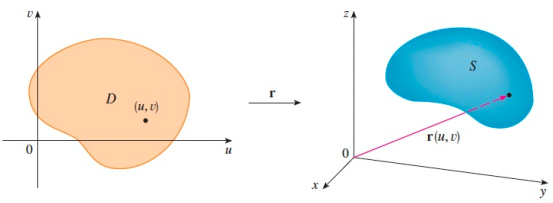
\includegraphics[scale=0.6]{images/13-parametric.png}
    \end{center}
\end{itemize}
\begin{example} $\textbf{r}(u,v) = (u,v,1-u-v)$, $(u,v)\in \mathbb{R}^2$. 
\begin{itemize}
    \item This is the plane $x+y+z = u + v + (1-u-v) = 1$.
    \item We can also view it as 
    \begin{align*}
        (u,v,1-u-v) 
        &= (0,0,1) + (u,0,-u) + (0,v,-v) = (0,0,1) + u(1,0,-1) + v(0,1,-1), \quad (u,v)\in \mathbb{R}^2.
    \end{align*}
    In this way, the plane is the one containing $(0,0,1)$ and all vectors in the planes generated by $(1,0,-1)$ and $(0,1,-1)$.
\end{itemize}
\end{example}


\begin{example} $\textbf{r}(u,v) = (2\cos u, v, 2\sin u)$, $u\in [0,2\pi], v\in \mathbb{R}$. 
\begin{itemize}
    \item Look at $x = 2\cos u, y = v, z = 2\sin u$, thus $x^2+z^2 = 4$, while $y\in \mathbb{R}$. This is a cylinder.
\end{itemize}
    \begin{center}
        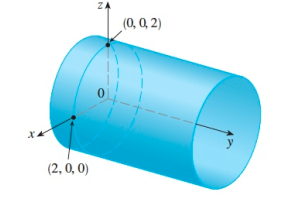
\includegraphics[scale=0.7]{images/13-ex2.png}
    \end{center}
\end{example}

\clearpage

\begin{example} $\textbf{r}(u,v) = (2\cos u, v, 2\sin u)$, $u\in \left[0,\frac{\pi}{2}\right], v\in [0,3]$. 
\begin{itemize}
    \item Look at $x = 2\cos u, y = v, z = 2\sin u$, thus $x^2+z^2 = 4$, while $y\in \mathbb{R}$. This is a cylinder.
    \item Note the angle $\theta$ in the $Oxz$-plane is $\pi/4$, thus only a quarter of the $Oxz$-plane is covered. 
\end{itemize}
    \begin{center}
        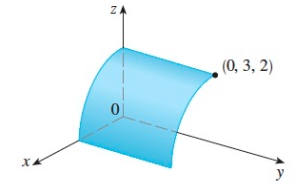
\includegraphics[scale=0.7]{images/13-ex3.png}
    \end{center}
\end{example}



\section{Parametrize a surface in $x,y,z$}
\begin{example} Find a parametric equation for $x^2+y^2 = 4, 0\leq z\leq 1$. 
\end{example}
\begin{proof} We can use polar coordinates $x = 2\cos \theta, y = 2\sin \theta$ and $0\leq z\leq 1$, thus 
\begin{equation*}
    r(\theta,z) = (2\cos \theta, 2\sin \theta, z)
\end{equation*}
The domain is $D = \{(\theta, z): 0\leq \theta \leq 2\pi, 0\leq z\leq 1\}$.
\end{proof}

\begin{example} Find a parametric equation for $z = 2\sqrt{x^2+y^2}, 0\leq z\leq 1$. 
\end{example}
\begin{proof}[Proof 1] We can just use the graph
\begin{equation*}
    r(x,y) = (x,y,z) = (x,y,2\sqrt{x^2+y^2}).
\end{equation*}
Note the condition $0\leq z\leq 1$ means $0\leq 2\sqrt{x^2+y^2}\leq 1$, thus $x^2+y^2 \leq \frac{1}{4}$. Therefore
    \begin{equation*}
        D = \left\{(x,y)\in \mathbb{R}^2: x^2+y^2 \leq \frac{1}{4}\right\}.
    \end{equation*}
\end{proof}

\begin{proof}[Proof 2] We can use polar coordinates $x = r\cos \theta, y = r\sin \theta$ and $0\leq z = 2r\leq 1$ which means $0\leq r\leq \frac{1}{2}$, thus 
\begin{equation*}
    \textbf{r}(\theta,z) = (r\cos \theta, r\sin \theta, 2r)
\end{equation*}
The domain now is 
\begin{equation*}
    D = \left\{(\theta, r): 0\leq \theta \leq 2\pi, 0\leq r\leq \frac{1}{2}\right\}.
\end{equation*}
\end{proof}


\section{Grid}
For a parametric surface $\textbf{r}(u,v)$, if we:
\begin{itemize}
    \item Fix $u=u_0$, run $v$ we get the images as a curvy grid on the surface
    \item Fix $v=v_0$, run $u$ we get the images as a curvy grid on the surface
\end{itemize}
The two direction at each point $(x_0,y_0,z_0) = r(u_0,v_0)$ form a tangent plane at that point. The two directions here are the partial derivatives
\begin{equation*}
    \textbf{r}_u \qquad \text{and} \qquad \textbf{r}_v.
\end{equation*}
The normal vector of the tangent plane is 
\begin{equation*}
    \textbf{n} = r_\textbf{u}\times r_\textbf{v} = 
    \left|
    \begin{array}{ccc}
         \textbf{i}& \textbf{j} & \textbf{k}  \\
         x_u &  y_u & z_u\\
         x_v &  y_v & z_v
    \end{array}
    \right|.
\end{equation*}
\begin{center}
    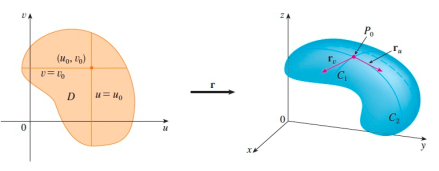
\includegraphics[scale=0.8]{images/13-grid.png}
\end{center}

\begin{example} Find the tangent plane of $x = u^2, y=v^2, z = u+2v$ at $(1,1,3)$.
\end{example}
\begin{proof} \quad 
\begin{itemize}
    \item Step 1. Solve for $(u,v)$: 
    \begin{equation*}
        \begin{cases}
            & x = u^2 = 1\\
            & y = v^2 = 1\\
            & z = u + 2v = 3
        \end{cases} \qquad\Longrightarrow\qquad \begin{cases}
            & u = \pm 1\\
            & v = \pm 1\\
            & u+2v = 3
        \end{cases} \qquad\Longrightarrow\qquad \begin{cases}
            u = 1\\
            v = 1
        \end{cases}
    \end{equation*}
    \item Step 2. Compute the partial derivatives of $\textbf{r}(u,v) = (u^2, v^2, u+2v)$
    \begin{align*}
        \textbf{r}_u = (2u, 0, 1)\\
        \textbf{r}_v = (0, 2v, 2).
    \end{align*}
    \item Step 3. Plug in the value $u=v=1$ to get 
    \begin{equation*}
        \begin{cases}
            \textbf{r}_u = (2, 0, 1)\\
            \textbf{r}_u = (0, 2, 2)
        \end{cases} 
    \end{equation*}
    \item Step 4. Compute the normal by cross product
    \begin{equation*}
        \textbf{n} = \textbf{r}_u \times \textbf{r}_v = 
        \left|
    \begin{array}{ccc}
         \textbf{i}& \textbf{j} & \textbf{k}  \\
         2 &  0 & 1\\
         0 &  2 & 2
    \end{array}
    \right| = (-2, -4, 4)
    \end{equation*}
    \item The tangent plane with normal $(-2,-4,-4)$ going through $(1,1,3)$ is
    \begin{equation*}
        \fbox{$\displaystyle 
        -2(x-1) - 4(y-1) - 4(z-3) = 0.
        $}
    \end{equation*}
\end{itemize}
\end{proof}


\begin{example} Find the tangent plane of $x = u^2+1, y=v^3+1, z = u+v$ at $(5,2,3)$.
\end{example}
\begin{proof} \quad 
\begin{itemize}
    \item Step 1. Solve for $(u,v)$: 
    \begin{equation*}
        \begin{cases}
            & x = u^2+1 = 5\\
            & y = v^3+1 = 2\\
            & z = u + v = 3
        \end{cases} \qquad\Longrightarrow\qquad \begin{cases}
            & u = 2 \\
            & v =  1.
        \end{cases} 
    \end{equation*}
    \item Step 2. Compute the partial derivatives of $\textbf{r}(u,v) = (u^2+1, v^3+1, u+v)$
    \begin{align*}
        \textbf{r}_u = (2u, 0, 1)\\
        \textbf{r}_v = (0, 3v^2, 1).
    \end{align*}
    \item Step 3. Plug in the value $u=2,  v=1$ to get 
    \begin{equation*}
        \begin{cases}
            \textbf{r}_u = (4, 0, 1)\\
            \textbf{r}_u = (0, 3, 1)
        \end{cases} 
    \end{equation*}
    \item Step 4. Compute the normal by cross product
    \begin{equation*}
        \textbf{n} = \textbf{r}_u \times \textbf{r}_v = 
        \left|
    \begin{array}{ccc}
         \textbf{i}& \textbf{j} & \textbf{k}  \\
         4 &  0 & 1\\
         0 &  3 & 1
    \end{array}
    \right| = (-3, -4, 12)
    \end{equation*}
    \item The tangent plane with normal $(-3,-4,12)$ going through $(5,2,3)$ is
    \begin{equation*}
        \fbox{$\displaystyle 
        -3(x-5) - 4(y-2) +12(z-3) = 0.
        $}
    \end{equation*}
\end{itemize}
\end{proof}
% % Lecture 16
\setcounter{section}{15}
\section{Lecture 16 - Tangent plane review and min/max of functions with several variables}

\subsection{Tangent plane revisited}
Given a surface with equation $F(x,y,z) = 0$, think of $x^2+\frac{y^2}{9}+\frac{z^2}{9}=1$ for example. 
\paragraph{Question.} Given a point $P_0(x_0,y_0,z_0)$ (think of $\left(\frac{1}{3},2,2\right)$ for example) that lies on the surface, find the tangent plane to the surface at the point $P_0$. 

\paragraph{Note.} To answer this question, we need to find a normal vector to the surface at $P_0$.

\paragraph{Method 1.} 
\begin{enumerate}
    \item Parametrize the surface by $\textbf{r}(u,v)$.
    \item Then solve for $(u_0,v_0)$ that corresponds to $P_0(x_0,y_0,z_0)$.
    \item Compute the normal vector by $\textbf{n} = \textbf{r}_u\times \textbf{r}_v$, let's say it is $(a,b,c)$.
    \item The tangent plane is $a(x-x_0)+b(y-y_0)+c(z-z_0) = 0$.
\end{enumerate}

\paragraph{Method 2.} 
\begin{enumerate}
    \item The normal is given by $\nabla F(x_0,y_0,z_0) = (F_x,F_y,F_z) = (a,b,c)$.
    \item The tangent plane is $a(x-x_0)+b(y-y_0)+c(z-z_0) = 0$.
\end{enumerate}
The second method is based on the fact that, if $\textbf{r}(t)=(x(t),y(t),z(t))$ is a curve in the surface passing through $P_0$, then 
\begin{equation*}
    F(x(t),y(t),z(t)) = 0 \qquad \Longrightarrow\qquad \frac{d}{dt}F(x(t),y(t),z(t)) = 0
\end{equation*}
Therefore 
\begin{equation*}
    (F_x,F_y,F_z)\cdot (x'(t),y'(t),z'(t)) = 0.  
\end{equation*}
Here $\textbf{r}'(t) = (x'(t),y'(t),z'(t))$ is a tangent vector to the curve, thus belongs to the tangent plane at $P_0$. In other words, $\nabla F$ is the normal vector to the tangent plane at $P_0$.

\begin{proof}[Proof using method 1] We can do
\begin{equation*}
    \begin{cases}
        x = \sin \phi \cos \theta \\
        \frac{y}{3} = \sin \phi \sin \theta \\
        \frac{z}{3} = \cos \phi
    \end{cases}
\end{equation*}
In other words,
\begin{equation*}
    r(\phi, \theta) = (\sin \phi \cos \theta , 3\sin \phi \sin \theta, 3\cos\phi).
\end{equation*}
To solve for $(\phi,\theta)$ at the point $P_0\left(\frac{1}{3}, 2,2\right)$ we solve
\begin{equation*}
    \begin{cases}
        \sin \phi\cos \theta &= \frac{1}{3}\\
        \sin \phi\sin \theta &= \frac{2}{3}\\
        \cos \phi &= \frac{2}{3}
    \end{cases}\qquad\Longrightarrow\qquad 
    \begin{cases}
    \sin\phi = \frac{\sqrt{5}}{3}    \\
    \cos\theta = \frac{1}{\sqrt{5}}\\
    \sin\theta = \frac{2}{\sqrt{5}}
    \end{cases}
\end{equation*}
We have 
\begin{equation*}
\begin{aligned}
    \textbf{r}_\phi &= (\cos \phi \cos\theta, 3\cos\phi\sin\theta, -3\sin\phi)  \\
    \textbf{r}_\theta &= (-\sin \phi \sin\theta, 3\sin\phi\cos\theta, 0)  \\
\end{aligned} 
\end{equation*}
We compute the normal vector
\begin{equation*}
\begin{aligned}
    \textbf{n} 
    &= 
    \left|
    \begin{array}{ccc}
         i & j & k  \\
         \cos \phi \cos\theta &  3\cos\phi\sin\theta & -3\sin\phi\\
         -\sin \phi \sin\theta & 3\sin\phi\cos\theta & 0
    \end{array}
    \right|=\Big(9\sin^2\phi\cos\theta, 3\sin^2\phi\sin \theta, 3\sin\phi\cos\phi\Big)\\
    &= \left(9\times \frac{5}{9}\times \frac{1}{\sqrt{5}}, 3\times \frac{5}{9} \times \frac{2}{\sqrt{5}}, 3 \times \frac{\sqrt{5}}{3}\times \frac{2}{3}\right) 
    = \left(\sqrt{5}, \frac{2\sqrt{5}}{3}, \frac{2\sqrt{5}}{3}\right).
\end{aligned}
\end{equation*}
We can simplify by choosing
\begin{equation*}
    \textbf{n} = \left(1,\frac{2}{3}, \frac{2}{2}\right)
\end{equation*}
and the tangent plane at $P\left(\frac{1}{3}, 2,2\right)$ is
\begin{equation*}
    \fbox{$\displaystyle
    \left(x-\frac{1}{3}\right) + \frac{2}{3} \left(y-2\right) + \frac{2}{3} \left(z-2\right) = 0.
    $}
\end{equation*}
\end{proof}

\begin{proof}[Proof using method 2] We have
\begin{equation*}
    \nabla F(x,y,z) = \left(2x, \frac{2y}{9}, \frac{2z}{9}\right) \qquad\Longrightarrow\qquad \textbf{n} = \nabla F\left(\frac{1}{3}, 2,2\right) = \left(\frac{2}{3}, \frac{4}{9},\frac{4}{9}\right). 
\end{equation*}
We can choose the parallel vector
\begin{equation*}
    \textbf{n} = \left(1, \frac{2}{3}, \frac{2}{3}\right)
\end{equation*}
and thus at $P\left(\frac{1}{3}, 2,2\right)$ we get the tangent plane
\begin{equation*}
    \fbox{$\displaystyle
    \left(x-\frac{1}{3}\right) + \frac{2}{3} \left(y-2\right) + \frac{2}{3} \left(z-2\right) = 0.
    $}
\end{equation*}
\end{proof}

\subsection{Critical points, local min, local max and saddle points}
% 
% Lecture 17
\setcounter{section}{16}
\section{Maximum and Minimum of functions on a domain with boundary}

Given $f(x,y):D\subset \mathbb{R}^2\to \mathbb{R}$. To find max/min on $D$ we follows the following steps (mostly from the previous lecture). 
\begin{enumerate}
    \item Find critical points (points where $\nabla f(x,y) = (0,0)$ or it does not exists)
    \begin{equation*}
        \text{Solve for}\;\nabla f(x,y) = 0.
    \end{equation*}
    \item Classify local max/min or saddle point (\emph{This step can be skipped if we only care about absolute max/min of the function}) 
    \begin{equation*}
        D = \left|\begin{array}{cc}
             f_{xx} & f_{xy}  \\
             f_{yx} & f_{yy} 
        \end{array}\right| = f_{xx}f_{yy} - f_{xy}^2 \qquad 
        \Longrightarrow\qquad 
        \begin{cases}
            D < 0: &\text{saddle point}    \\
            D = 0: &\text{inconclusive}    \\
            D > 0 
            & 
            \begin{cases}
            f_{xx} > 0 &\text{local min}\\
            f_{xx} < 0 &\text{local max}.
            \end{cases}
        \end{cases}
    \end{equation*}
    \item Find max/min on the boundary. 
    \begin{enumerate}
        \item Draw a graph to identify parts of the boundary.
        \item On each part, write the relation between $x$ and $y$, use that to simplify $f(x,y)$ into a function of one variable $g(x)$ or $g(y)$, together with the domain of $x$ and $y$ correspondingly.
        \item Use Cal 2 to find max/min of this one-variable function. 
    \end{enumerate}
    \item Compare all the max/min values found in Step 3 and the values of all critical points in Step 1. The biggest is the absolute max, the smallest is the absolute min.
\end{enumerate}

\paragraph{Notes.} When the question is finding absolute maximum or absolute minimum, we can ignore step 2 completely. 

\clearpage

\begin{example}
    Find the absolute max/min values for $f(x,y) = x+y$ on the region $D$ given by the picture below below.
    \begin{equation*}
        D = \{(x,y)\in \mathbb{R}^2: x^2\leq y\leq 3\}.
    \end{equation*}
\end{example}

\begin{center}
    \begin{tikzpicture}[
    declare function={
        a=-3;
        b=3;
        f(\x)=\x^2-1;
        g(\x)=3;
        }]
    \pgfmathsetmacro{\sqrtofthree}{sqrt(3)} % Calculate sqrt(3)
    \begin{axis}[
        axis lines=middle,
        axis on top,
        xlabel=$x$,
        ylabel=$y$,
        xmin=-4,xmax=4,ymin=-2,ymax=4,
        ytick={-1,0,1,2,3},
        xtick={-4,-3,-2,-1,0,1,2,3,4},
        % xticklabels={$a$,$1$,$b$}, 
        % https://tex.stackexchange.com/a/68407/121799
        every axis x label/.style={at={(current axis.right of origin)},anchor=north west},
        every axis y label/.style={at={(current axis.above origin)},anchor=north east}]
        \addplot[name path=A,blue,thick,domain=-4:4,smooth] {f(x)};
        \addplot[name path=C,blue,thick,domain=-3:3,smooth] {g(x)};
        \path[name path=B] (\pgfkeysvalueof{/pgfplots/xmin},0) -- (\pgfkeysvalueof{/pgfplots/xmax},0);
      \addplot [gray!30] fill between [
            of=A and C,
            % soft clip={domain= -\sqrtofthree:\sqrtofthree},
            soft clip={domain= -2:2},
        ];
        \addplot [gray] fill between [
            of=A and C,soft clip={domain=1:b},
        ];
        \path 
        ({-1},{3+0.3}) node{$D_1$}
        ({-1.8},{1}) node{$D_2$}
        ({1},{1.5}) node{$D$};
    \end{axis}
\end{tikzpicture}
\end{center}

\begin{proof}\quad 
\begin{enumerate}
    \item Finding the intersection of $y=x^2-1$ and $y=3$, we have $x^2-1 = 3$, thus $x^2 = 4$, hence $x=2$ or $x=-2$.
    \item Critical points: $\nabla f(x,y) = (1,1)$. Solving for $\nabla f(x,y) = (0,0)$ does not yield any solution as      $(1,1) = (0,0)$
    has no solution $(x,y)$. We conclude that there is no critical point. 
    \item Find max/min on the boundary: there are two parts of the boundary:
    \begin{itemize}
        \item On $D_1$, we have $y=-3$ and $-2\leq x\leq 2$, and 
        \begin{align*}
            f(x,y) = x+y = x+3 \qquad \Longrightarrow\qquad \begin{cases}
                \text{max}\; 5\;\text{at}\;(2,3)\\
                \text{min}\; 1\;\text{at}\;(-2,3).
            \end{cases}
        \end{align*}
        \item On $D_2$, we have $y=x^2-1$ and $-2\leq x\leq 2$, and 
        \begin{align*}
            f(x,y) = x+ y = x+ x^2-1 = g(x).
        \end{align*}
        This is now a separate question: \fbox{$\displaystyle
            \text{Find max/min}\;g(x) = x^2+x-1\;\text{over}\;x\in [-2,2].
            $}
        \begin{itemize}
            \item $g'(x) = 0$ iff $2x+1 = 0$, iff $x=-\frac{1}{2}$. The corresponding $y = x^2-1 = \left(-\frac{1}{2}\right)^2-1 = -\frac{3}{4}$.
            
            We compute $g\left(-\frac{1}{2}\right) = \left(-\frac{1}{2}\right)^2 + \left(- \frac{1}{2}\right) - 1 = -\frac{5}{4}$, and $(x,y) = \left(-\frac{1}{2}, -\frac{3}{4}\right)$. 
            \item If $x=-2$ then $y=3$, 
            $g(-2) = (-2)^2+(-2)-1 = 1$, at $(-2,3)$.
            \item If $x=2$ then $y=3$, 
            $g(2) = (2)^2+(2)-1 = 5$, at $(2,3)$.
        \end{itemize}
    \end{itemize}
    \item Comparing all points, we conclude 
    \begin{itemize}
        \item Absolute max $=5$ at $(2,3)$.
        \item Absolute min $=-\frac{5}{4}$ at $\left(-\frac{1}{2}, -\frac{3}{4}\right)$.
    \end{itemize}
\end{enumerate}
\end{proof}


\clearpage
\begin{example}
    Find the absolute max/min values for $f(x,y) =x^2-2xy+2y$ on the region $D$ given by the picture below below.
    \begin{equation*}
        D = \{(x,y)\in \mathbb{R}^2: 0\leq x\leq 3, 0\leq y\leq 2\}.
    \end{equation*}
\end{example}

\clearpage

\begin{example}
    Find the absolute max/min values for $f(x,y) =2+2x+2y-x^2-y^2$ on the triangular region in the first quadrant bounded by and including $y=9-x$.
\end{example}


\clearpage
\begin{example} Let $f(x,y)=2x^2-y^2+6y$ on the disk $D$ given by $x^2+y^2\leq 16$.
    \begin{itemize}
        \item[(a)] Find all critical points of $f$.
        % \item[(b)] Find the function values of $f$ on the boundary of $D$.
        \item[(b)] Find the absolute max/min of $f$ on $D$. 
    \end{itemize}
\end{example}
% 
\setcounter{section}{17}
\section{Lagrange multipliers}
To find max/min of $f(x,y,z)$ with a given constraint $g(x,y,z)=0$. 
\begin{enumerate}
    \item We find solutions for $(x,y,z)$ and any possible $\lambda$ that satisfy
    \begin{equation*}
        \begin{cases}
        \begin{aligned}
            \nabla f(x,y,z) &= \lambda \nabla g(x,y,z) \\
                   g(x,y,z) &= 0.
        \end{aligned}
        \end{cases}
    \end{equation*}
    \item Among all $(x,y,z)$ we found, find the biggest or smallest values of $f(x,y,z)$. They are potential absolute max/min of $f$ given the constraint $g$.
\end{enumerate}

\begin{example} Find max/min $f(x,y) = x^2+y^2$ subjected to $xy=1$. 
\end{example}
\begin{proof} Here $f(x,y) = x^2+y^2$ and $g(x,y) = xy-1$. 
\begin{equation*}
    \begin{cases}
        \begin{aligned}
            \nabla f(x,y) &= \lambda \nabla g(x,y)\\
            g(x,y) &= 0
        \end{aligned}
    \end{cases} \qquad\Longrightarrow\qquad 
    \begin{cases}
        \begin{aligned}
            (2x, 2y) &= \lambda(y,x)\\
            xy&=1
        \end{aligned}
    \end{cases} \qquad\Longrightarrow\qquad \begin{cases}
        2x&=\lambda y\\
        2y&=\lambda x\\
        xy &= 1
    \end{cases}
\end{equation*}
If we multiply the two equations together side by side, then
\begin{equation*}
    4xy = \lambda^2 xy \qquad\Longrightarrow\qquad \lambda^2 = 4.
\end{equation*}
\begin{itemize}
    \item If $\lambda=2$ then $x=y$ and $xy=1$, thus $(x,y)=(1,1)$ or $(-1,-1)$.
    \item If $\lambda=-2$ then $x=-y$, then $-x^2=1$ has no solution.
\end{itemize}
We conclude that the minimum of $f$ is $2$, at $(1,1)$ or $(-1,-1)$. Here $f$ has no max since if we choose 
\begin{equation*}
    (x,y) = \left(n,\frac{1}{n}\right) \qquad\Longrightarrow\qquad f(x,y) = n^2+\frac{1}{n^2} \geq n^2 \to \infty
\end{equation*}
if we let $n\to \infty$.
\end{proof}

\begin{example}  Find max/min $f(x,y) = x^2+2y^2$ subjected to $x^2+y^2=1$. 
\end{example}

\begin{proof} Here $f(x,y) = x^2+2y^2$ and $g(x,y) = x^2+y^2$. 
\begin{equation*}
    \begin{cases}
        \begin{aligned}
            \nabla f(x,y) &= \lambda \nabla g(x,y)\\
            g(x,y) &= 0
        \end{aligned}
    \end{cases} \qquad\Longrightarrow\qquad 
    \begin{cases}
        \begin{aligned}
            (2x, 4y) &= \lambda(2x,2y)\\
            x^2+y^2&=1
        \end{aligned}
    \end{cases} \qquad\Longrightarrow\qquad \begin{cases}
    \begin{aligned}
        2x&=\lambda 2x\\
        4y&=\lambda 2y\\
        x^2+y^2&=1
        \end{aligned}
    \end{cases}
\end{equation*}
Look at the first equation, we have $2x(1-\lambda) = 0$. 
\begin{itemize}
    \item If $x=0$ then $y^2=1$, thus $(x,y) = (0,1), (0,-1)$.
    \item If $x\neq 0$ then $\lambda = 1$, then the second equation reads $4y = 2y$, thus $y=0$ and hence $x^2=1$, thus $(x,y)=(1,0), (-1,0)$.
\end{itemize}
Comparing the values, we have $f$ is max $2$ at $(0,1)$ or $(0,-1$, and $f$ is min $1$ at $(1,0)$ or $(-1,0)$.
\end{proof}

\begin{example} A rectangular box without a lid is to be made from $12\;\mathrm{m}^2$ of cardboard. Find the maximum volume of such a box.
\end{example}
\begin{proof} Let $x,y$ be the measurements of the two sides on the bottom, and $z$ be the height of the box. Here the volume is 
\begin{equation*}
    f(x,y,z) = xyz,    
\end{equation*}
and the area of the box without the lid is $xy + 2xz + 2yz = 12$, thus the constraint is
\begin{equation*}
    g(x,y,z) = xy + 2xz + 2yz -12 = 0.
\end{equation*}
The system is
\begin{equation*}
\begin{cases}
    \nabla f(x,y,z) = \lambda \nabla g(x,y,z)\\
    g(x,y,z) = 0
\end{cases}
     \qquad \Longrightarrow\qquad  
     \begin{cases}
         (yz, xz, xy) =\lambda (y+2z, x+2z, 2x+2y)\\
         xy + 2xz + 2yz = 12.
     \end{cases}
\end{equation*}
Therefore
\begin{equation*}
    \begin{cases}
    \begin{aligned}
        yz &= \lambda(y+2z)\\
        xz &= \lambda(x+2z)\\
        xy &= \lambda(2x+2y)\\
        xy + 2xz + 2yz &= 12.
    \end{aligned}
    \end{cases}
\end{equation*}
If $\lambda = 0$ then $yz=xz=xy = 0$, which does not satisfy $xy + 2xz + 2yz = 12$. We can safely assume $x,y,z\neq 0$ as they are dimensions of the box. Thus by dividing the equations side by side we have 
\begin{equation*}
    \begin{cases}
    \begin{aligned}
        x\times yz &= x\times \lambda(y+2z)\\
        y\times xz &= y\times\lambda(x+2z)\\
        z\times xy &= z\times\lambda(2x+2y)\\
        xy + 2xz + 2yz &= 12.
    \end{aligned}
    \end{cases} \qquad\Longrightarrow\qquad 
    \begin{cases}
        \begin{aligned}
            xyz &= \lambda (xy + 2xz)\\
            xyz &= \lambda (xy + 2yz)\\
            xyz &= \lambda (2xz + 2yz)\\
            xy + 2xz + 2yz &= 12.
        \end{aligned}
    \end{cases}
\end{equation*}
Therefore, from the 1st and 2nd equation (use $\lambda\neq 0$ and $z\neq 0$)
\begin{equation*}
    xy +2xz = xy + 2yz \qquad\Longrightarrow\qquad 2xz=2yz \qquad\Longrightarrow\qquad x=y.
\end{equation*}
from the 2nd and 3rd equation (use $\lambda\neq 0$ and $z\neq 0$)
\begin{equation*}
    xy +2yz = 2xz + 2yz \qquad\Longrightarrow\qquad xy=2xz \qquad\Longrightarrow\qquad y=2x.
\end{equation*}
Therefore 
\begin{equation*}
    x = y = 2z.
\end{equation*}
Use this 
\end{proof}


\noindent 
Let 
\begin{equation*}
    \V(\x) = 2-\sin(2\pi x) - \sin(2\pi y), \qquad \x = (x,y)\in \T^2.
\end{equation*}
We are interested in estimating, for $\mu>0$ and $\gamma > 0$ the Sobolev norm $H^{2+s}(\T^2)$ of the function
\begin{equation*}
    \K_\mu(\x) = (\mu + \V(\x))^{{-1/2}}, \qquad \x\in \T^2.
\end{equation*}

\section{Evaluate the $3rd$-derivative}
We want to compute 
\begin{align*}
    \partial^2_{x_ix_j} \K_\mu(\x) 
    &= \frac{3\gamma^2}{4}\left(\mu+\V(\x)^\gamma\right)^{-5/2} 
        \left(\gamma \V^{\gamma-1} \V_{x_i}\right)
        \left(\gamma \V^{\gamma-1} \V_{x_j}\right) \\
    & -\frac{1}{2}(\mu + \V^\gamma)^{-3/2} 
        \left(
            \gamma(\gamma-1)\V^{\gamma-2}
            \V_{x_i}\V_{x_j}
            + 
            \gamma\V^{\gamma-1} \V_{x_ix_j}
        \right).
\end{align*}
We have 
\begin{align*}
    \partial_{x_k}\Big(\partial^2_{x_ix_j} \K_\mu(\x) \Big) = I_1 + I_2 + I_3 + I_4,
\end{align*}
where
\begin{align*}
    I_1 &= -\frac{15\gamma^2}{8} (\mu+\V^\gamma)^{-7/2} \prod_{i,j,k} \left(\gamma\V^{\gamma-1}\V_{x_i}\right) \\
    I_2 &= \frac{3\gamma^2}{4}(\mu+\V^\gamma)^{-5/2} \frac{\partial}{\partial_{x_k}} 
    \left(\gamma\V^{\gamma-1}\V_{x_i}\right)
    \left(\gamma\V^{\gamma-1}\V_{x_j}\right)\\
    I_3 &= \frac{3}{4}(\mu+\V^\gamma)^{-5/2} 
        \left( 
            \gamma\V^{\gamma-1}\V_{x_k} 
        \right)
        \left(
            \gamma(\gamma-1)\V^{\gamma-2}\V_{x_i}\V_{x_j}
            + 
            \gamma\V^{\gamma-1} \V_{x_ix_j}
        \right) \\
    I_4 &= -\frac{1}{2}(\mu+\V^\gamma)^{-3/2} \frac{\partial}{\partial x_k}
    \left(
        \gamma(\gamma-1)\V^{\gamma-2}
        \V_{x_i}\V_{x_j}
        + 
        \gamma\V^{\gamma-1} \partial^2_{x_ix_j}\V
    \right). 
\end{align*}

We only need to differentiate $I_2$ and $I_4$. 
\subsection{Compute $I_1$} We have
\begin{align*}
\fbox{$\displaystyle
    I_1 \leq \frac
    {
        |\x-\x_0|^{6\gamma-3}
    }
    {
        (\mu+|\x-\x_0|^{2\gamma})^{7/2}
    }
$}.
\end{align*}

\subsection{Compute $I_2$}
We have
\begin{align*}
    &\frac{\partial}{\partial_{x_k}} 
    \left(\gamma\V^{\gamma-1}\V_{x_i}\right)
    \left(\gamma\V^{\gamma-1}\V_{x_j}\right) = \\
    & \qquad 
        \Big[ 
        \gamma(\gamma-1)\V^{\gamma-2} \V _{x_i}\V_{x_k}
        + 
        \gamma  \V^{\gamma-1} \V_{x_ix_k}
        \Big] \left(\gamma\V^{\gamma-1}\V_{x_j}\right)  
        \color{red} 
            \sim \left(|\x-\x_0|^{2\gamma-2} + |\x-\x_0|^{2\gamma-2}\right)|\x-\x_0|^{2\gamma-1}
        \color{black} \\
    & \qquad \qquad + \\    
    & \qquad  
        \Big[ 
        \gamma(\gamma-1)\V^{\gamma-2} \V_{x_j}\V_{x_k}
        + 
        \gamma  \V^{\gamma-1}\V_{x_jx_k}
        \Big] \left(\gamma\V^{\gamma-1}\V_{x_i}\right). 
\end{align*}
Therefore
\begin{align*}
    I_2 &= \frac{3\gamma^2}{4}(\mu+\V^\gamma)^{-5/2} \\
    & 
    \left(
        \Big[ 
        \gamma(\gamma-1)\V^{\gamma-2}\V_{x_i}
        + 
        \gamma  \V^{\gamma-1} \V_{x_ix_k}
        \Big] 
        \left(\gamma\V^{\gamma-1}\V_{x_j}\right)
        + 
        \Big[ 
        \gamma(\gamma-1)\V^{\gamma-2} \V _{x_j}
        + 
        \gamma  \V^{\gamma-1} \V_{x_jx_k}
        \Big] \left(\gamma\V^{\gamma-1}\V_{x_i}\right) 
    \right)
\end{align*}
And thus
\begin{align*}
    I_2 \leq 
    \frac{
        |\x-\x_0|^{2\gamma-2} \cdot |\x-\x_0|^{2\gamma-1} 
    }{(\mu+|\x-\x_0|^{2\gamma})^{5/2}} 
    = 
\fbox{$ \displaystyle 
    \frac{
        |\x-\x_0|^{4\gamma-3}
    }
    {
        (\mu+|\x-\x_0|^{2\gamma})^{5/2}
    }
$}
\end{align*}
\subsection{Compute $I_3$}
We have
\begin{align*}
    I_3 \leq 
    \frac
    {
        |\x-\x_0|^{2\gamma-1} \cdot 
        \Big(
            |\x-\x_0|^{2\gamma-2} + |\x-\x_0|^{2\gamma-2}
        \Big)
    }
    {   
        (\mu+|\x-\x_0|^{2\gamma})^{5/2}
    } 
    = 
    \fbox{$ \displaystyle
    \frac
    {
        |\x-\x_0|^{4\gamma-3}
    }
    {
        (\mu+|\x-\x_0|^{2\gamma})^{5/2}
    }
    $}. 
\end{align*}
\subsection{Compute $I_4$} We have
\begin{align*}
    I_4 &= -\frac{1}{2}(\mu+\V^\gamma)^{-3/2} 
    \left(
        \gamma(\gamma-1) \sum_{i,j,k} \V^{\gamma-2} \V_{x_ix_j}\V_{x_k} 
        +
        \gamma \V^{\gamma-1} \V_{x_ix_jx_k} 
        +
        \gamma(\gamma-1)(\gamma-2)\V^{\gamma-3} \V_{x_i}\V_{x_j}\V_{x_k}
    \right).
\end{align*}
Therefore 
\begin{align*}
    I_4 \leq \frac
            {
                |\x-\x_0|^{2\gamma-3} + |\x-\x_0|^{2\gamma-1} + |\x-\x_0|^{2\gamma-3}
            }
            {
                (\mu+|\x-\x_0|^{2\gamma})^{3/2}
            }
            \leq 
            \fbox{$\displaystyle
                \frac{|\x-\x_0|^{2\gamma-3}}
                {(\mu+|\x-\x_0|^{2\gamma})^{3/2}}
                + 
                \frac{|\x-\x_0|^{2\gamma-1}}
                {(\mu+|\x-\x_0|^{2\gamma})^{3/2}}
            $}. 
\end{align*}
\subsection{Putting everything together}
We obtain
\begin{align*}
    I_1+I_2+I_3+I_4 \leq  
                \frac
                {
                    |\x-\x_0|^{6\gamma-3}
                }
                {
                    (\mu+|\x-\x_0|^{2\gamma})^{7/2}
                }
    + 
                 \frac
                {
                    |\x-\x_0|^{4\gamma-3}
                }
                {
                    (\mu+|\x-\x_0|^{2\gamma})^{5/2}
                }
    + 
    \frac
                {
                    |\x-\x_0|^{2\gamma-3}
                }
                {
                    (\mu+|\x-\x_0|^{2\gamma})^{3/2}
                }
    + 
    \frac
                {
                    |\x-\x_0|^{2\gamma-1}
                }
                {
                    (\mu+|\x-\x_0|^{2\gamma})^{3/2}.
                }
\end{align*}
Therefore, we have
\begin{align*}
    &\int_{\T^2} |D^3\K_\mu(\x)|^2\;d\x \\
    &\qquad 
    \leq C
    \left(
        1 
        + 
        \int_0^1 \frac{r^{12\gamma-5}}{(\mu+r^{2\gamma})^7}\;dr 
        + 
        \int_0^1 \frac{r^{8\gamma-5}}{(\mu+r^{2\gamma})^5}\;dr 
        +
        \int_0^1 \frac{r^{4\gamma-5}}{(\mu+r^{2\gamma})^3}\;dr 
        +
        \int_0^1 \frac{r^{4\gamma-1}}{(\mu+r^{2\gamma})^3}\;dr 
    \right)\\
    &\qquad 
    \leq C 
    \left(
        1 
        + 
        \mu^{-1-\frac{2}{\gamma}}\int_0^{\mu^{-\frac{1}{2\gamma}}} \frac{s^{12\gamma-5}\;ds}{(1+s^{2\gamma})^7}
        + 
        \mu^{-1-\frac{2}{\gamma}}\int_0^{\mu^{-\frac{1}{2\gamma}}} \frac{s^{8\gamma-5}\;ds}{(1+s^{2\gamma})^5} 
        + 
        \mu^{-1-\frac{2}{\gamma}}\int_0^{\mu^{-\frac{1}{2\gamma}}} \frac{s^{4\gamma-5}\;ds}{(1+s^{2\gamma})^3} 
        \right. \\
    &\qquad \qquad\qquad\qquad \qquad\qquad 
     \qquad \qquad\qquad\qquad \qquad\qquad\qquad
        \left. 
        + 
        \mu^{-1}\int_0^{\mu^{-\frac{1}{2\gamma}}} \frac{s^{4\gamma-1}\;ds}{(1+s^{2\gamma})^3} 
    \right) \\
    &\qquad \leq C\left(1 + \mu^{-1-\frac{2}{\gamma}} + \mu^{-1}\right).
\end{align*}

\end{document}